\section{Zarządzanie towarami}
Magazynier jest osobą odpowiedzialną za odwzorowanie aktualnego stanu
magazynu w systemie. Wprowadza dane towarów do systemu, a także
aktualizuje ich stan. Ponadto zarządza on dokumentacją przyjęć towaru (PZ) do
magazynu oraz danymi kontrahentów. W razie potrzeby może zwrócić
przyjęty towar oraz skorygować aktualny stan towaru 
(np. gdy towar straci swój termin ważności). Diagram przedstawiający opisane przypadki użycia
został zaprezentowany na rysunku \ref{fig:ZarzadzanieTowarami}.

\begin{figure}[H]
  \centering
  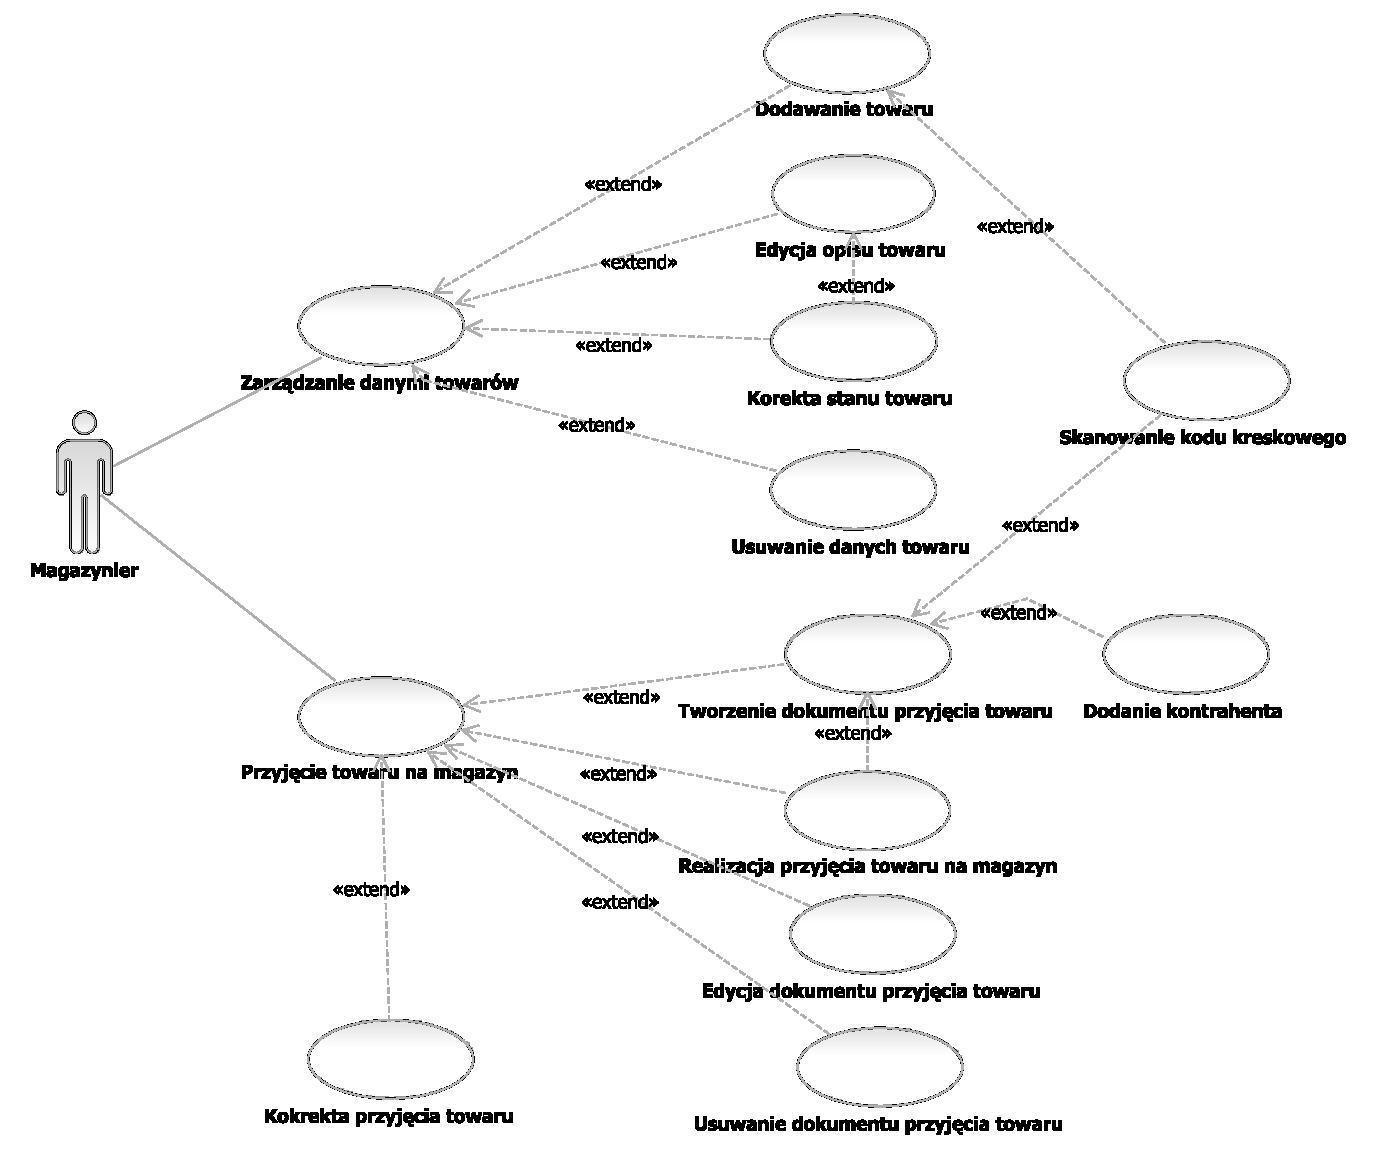
\includegraphics[scale=0.6]{../img/usecase/ZarzadzanieTowarami.pdf}
  \caption{Diagram przypadków użycia dla zarządzania towarami.}
  \label{fig:ZarzadzanieTowarami}
\end{figure}

\newpage
\singlespacing
\subsection{Zarządzanie danymi towarów}

\begin{usecase}
  \addtitle{PU18}{Zarządzanie danymi towarów}
  \addfield{Priorytet:}{wysoki}
  \addfield{Aktor główny:}{Magazynier}
  \addfield{Warunki początkowe:}{Aktor został uwierzytelniony.}
  % Warunki końcowe (brak).
  \addscenario{Scenariusz główny:}{
  \item Aktor wybiera opcję przeglądania listy towarów w magazynie.
  \item System wyświetla listę towarów w magazynie wraz z opcjami zarządzania danymi dokumentów.
  }
  \addfield{Wymagania funkcjonalne:}{2.}
\end{usecase}

\begin{figure}[H]
  \centering
  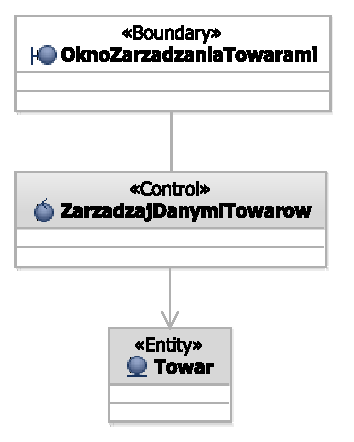
\includegraphics[angle=\ecbangle, scale=\ecbscale]{../img/usecase/pu18ecb.pdf}
  \caption{\ecbcaption18}
\end{figure}
\newpage
\begin{figure}[H]
  \centering
  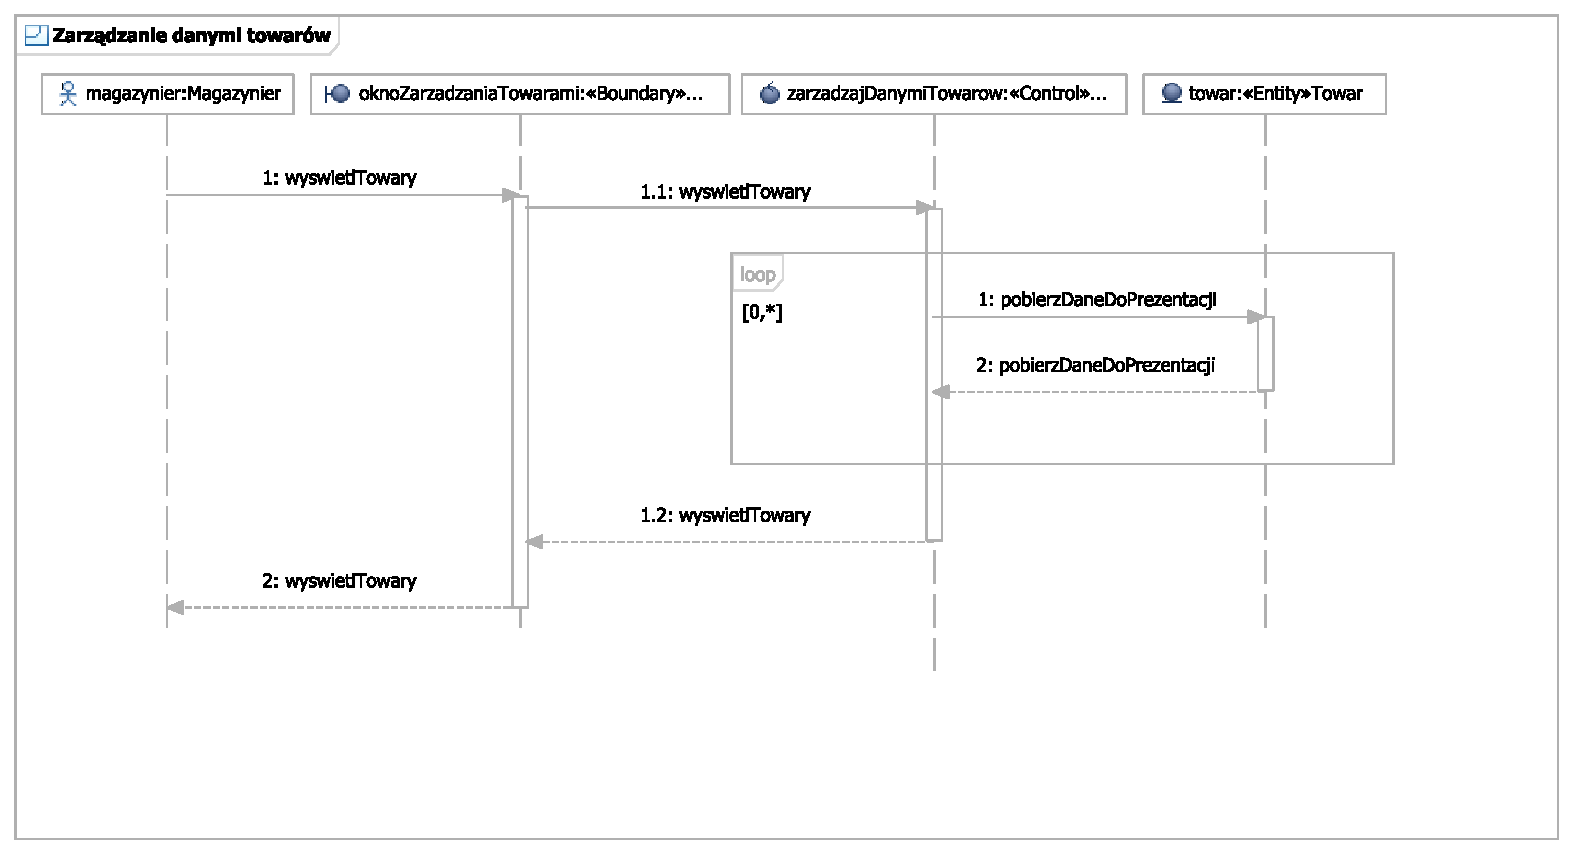
\includegraphics[angle=\seqangle, scale=\seqscale]{../img/usecase/pu18seq.pdf}
  \caption{\seqcaption18}
\end{figure}
\newpage

%%%%%%%%
\subsection{Dodawanie towaru}
%
\begin{usecase}
  \addtitle{PU19}{Dodawanie towaru}
  \addfield{Priorytet:}{wysoki}
  \addfield{Aktor główny:}{Magazynier}
  \addfield{Rozszerza przypadki:}{PU18}
  \addfield{Warunki początkowe:}{Aktor został uwierzytelniony.}
  \additemizedfield{Warunki końcowe:}{ 
    \item Dane towaru zostały zapisane w systemie.
    \item Użytkownik może wyświetlić dane towaru na liście towarów. % TODO jak warunki końcowe mają się do scenariuszy alternatywnych?
    \item Dane towaru mogą być uwzględnione w dokumentach przedstawionych w rozdziale \ref{dziedzina-problemu}.
  }
  \addscenario{Scenariusz główny:}{
    \item Aktor wybiera opcję dodania nowego towaru do systemu.
    \item System wyświetla formularz dodawania nowego towaru do systemu.
    \item Aktor wpisuje wymagane oraz opcjonalne dane do formularza.
    \item Aktor wybiera opcję zapisania nowego towaru w systemie.
    \item System informuje aktora, że towar został poprawnie zapisany w systemie.
  }
  \addscenario{Scenariusz alternatywny:} {
    \item [4.a] Aktor nie podał wymaganych pól formularza:
      \begin{enumerate}
        \item[1--4.] Jak w scenariuszu głównym.
        \item[5.] System wyświetla powiadomienie o konieczności podania wymaganych informacji.
        \item[6.] Aktor wraca do punktu 3.  
      \end{enumerate}
    \item [4.b] Aktor podał błędne wartości pól formularza:
      \begin{enumerate}
        \item[1--4.] Jak w scenariuszu głównym.
        \item[5.] System wyświetla powiadomienie o błędnych polach formularza.
        \item[6.] Aktor wraca do punktu 3.
      \end{enumerate}
  }
  \addfield{Zakres przetwarzanych danych:} {
    Dane towaru takie jak przedstawione w rozdziale \ref{dziedzina-problemu}.
  }
  \addfield{Warunki poprawności danych:}{
    Warunki poprawności takie jak przedstawione w rozdziale \ref{dziedzina-problemu}.
  }
  \addfield{Wymagania funkcjonalne:}{2.1}
\end{usecase}

\begin{figure}[H]
  \centering
  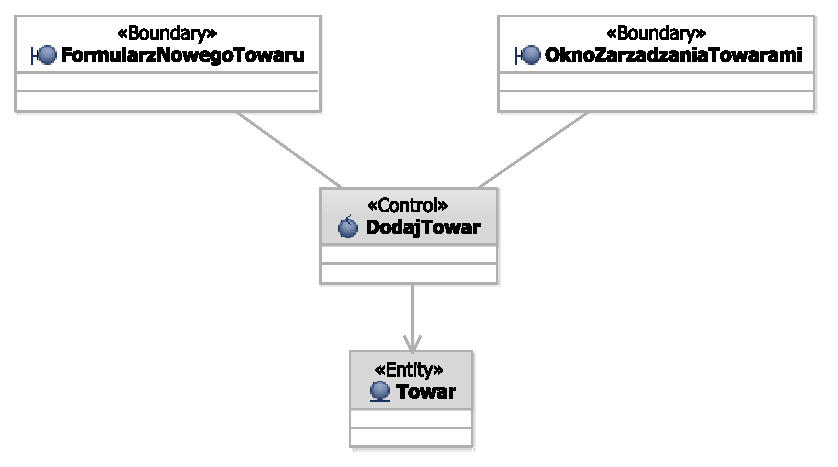
\includegraphics[angle=\ecbangle, scale=\ecbscale]{../img/usecase/pu19ecb.pdf}
  \caption{\ecbcaption19}
\end{figure}

\begin{figure}[H]
  \centering
  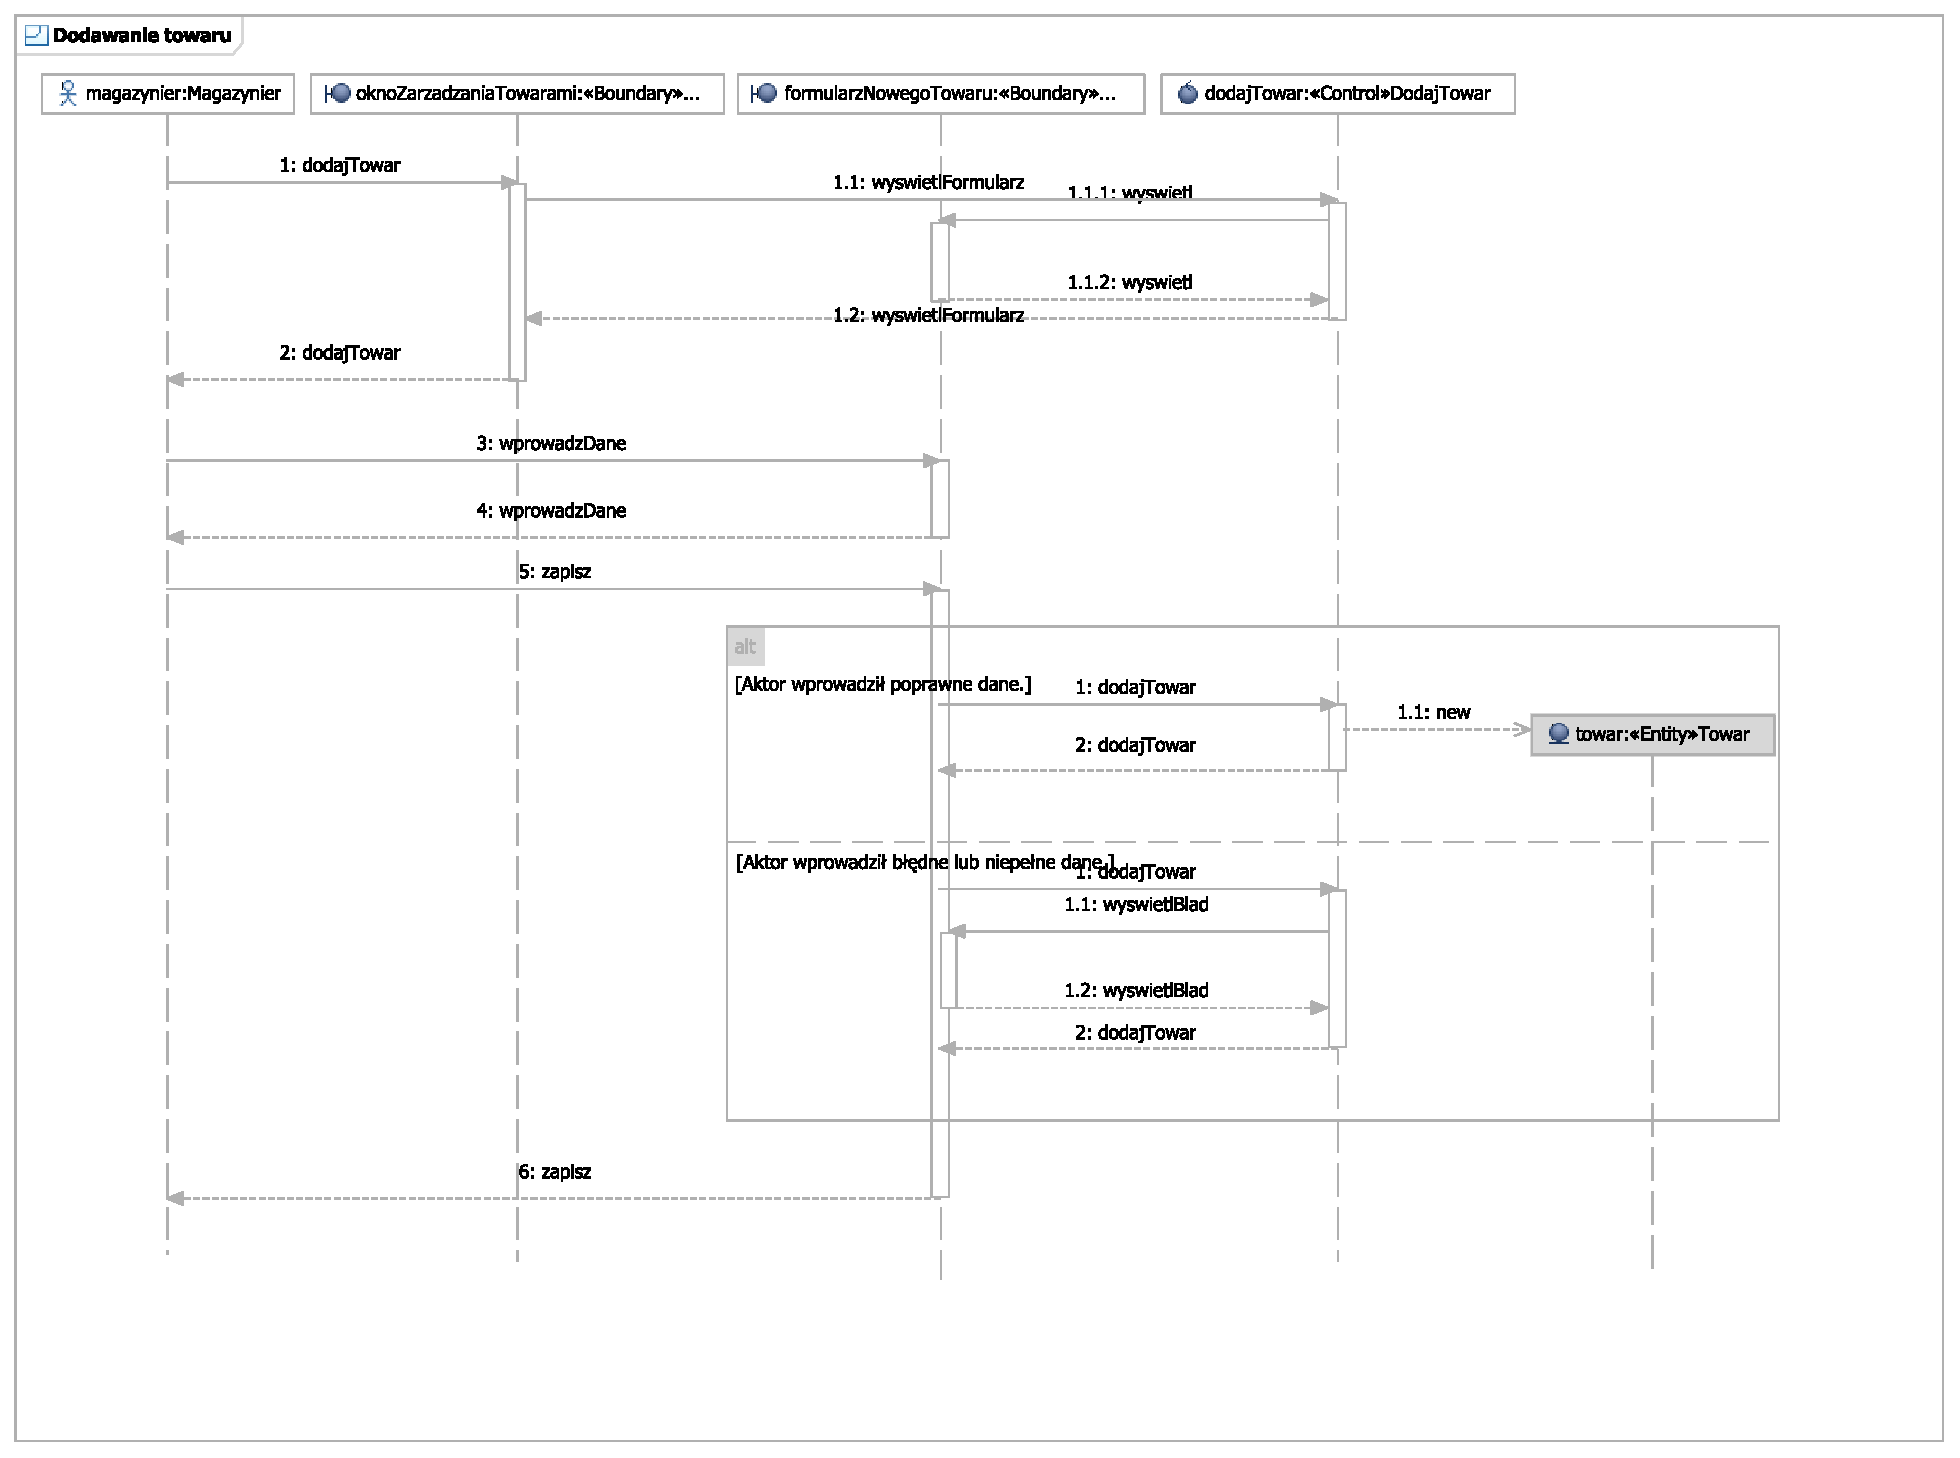
\includegraphics[angle=\seqangle, scale=0.5]{../img/usecase/pu19seq.pdf}
  \caption{\seqcaption19}
\end{figure}
\newpage

%%%%%%%
\subsection{Edycja opisu towaru}
\begin{usecase}
  \addtitle{PU20}{Edycja opisu towaru}
  \addfield{Priorytet:}{wysoki}
  \addfield{Aktor główny:}{Magazynier}
  \addfield{Rozszerza przypadki:}{PU18}
  \addfield{Warunki początkowe:}{Aktor został uwierzytelniony.}
   \additemizedfield{Warunki końcowe:}{ 
    \item Dane towaru zostały zaktualizowane w systemie.
    \item Użytkownik może wyświetlić dane towaru na liście towarów. 
    \item Dane towaru mogą być uwzględnione w dokumentach przedstawionych w rozdziale \ref{dziedzina-problemu}.
  }
  \addscenario{Scenariusz główny:}{
    \item Aktor wybiera opcję aktualizacji danych wskazanego towaru.
    \item System wyświetla formularz aktualizacji danych towaru wypełniony obecnymi danymi towaru.
    \item Aktor wypełnia lub zmienia wybrane pola formularza.
    \item Aktor wybiera opcję aktualizacji danych towaru.
    \item System informuje aktora, że dane towaru zostały poprawnie zaktualizowane.
  }
  % TODO duplikacja przebiegów alternatywnych z PU31
  \addscenario{Scenariusz alternatywny:} {
    \item [4.a] Aktor nie podał wymaganych pól formularza:
      \begin{enumerate}
        \item[1.--4.] Jak w scenariuszu głównym.
        \item[5.] System wyświetla powiadomienie o konieczności podania wymaganych informacji.
        \item[6.] Aktor wraca do punktu 3.  
      \end{enumerate}
    \item [4.b] Aktor podał błędne wartości pól formularza:
      \begin{enumerate}
        \item[1.--4.] Jak w scenariuszu głównym.
        \item[5.] System wyświetla powiadomienie o błędnych polach formularza.
        \item[6.] Aktor wraca do punktu 3.
      \end{enumerate}
  }
  \addfield{Zakres przetwarzanych danych:}{Dane towaru dostępne przy edycji, przedstawione w rozdziale \ref{dziedzina-problemu}.}
  \addfield{Warunki poprawności danych:}{Warunki poprawności takie jak przedstawione w rozdziale \ref{dziedzina-problemu}.}
  \addfield{Wymagania funkcjonalne:}{2.2}
\end{usecase}

\begin{figure}[H]
  \centering
  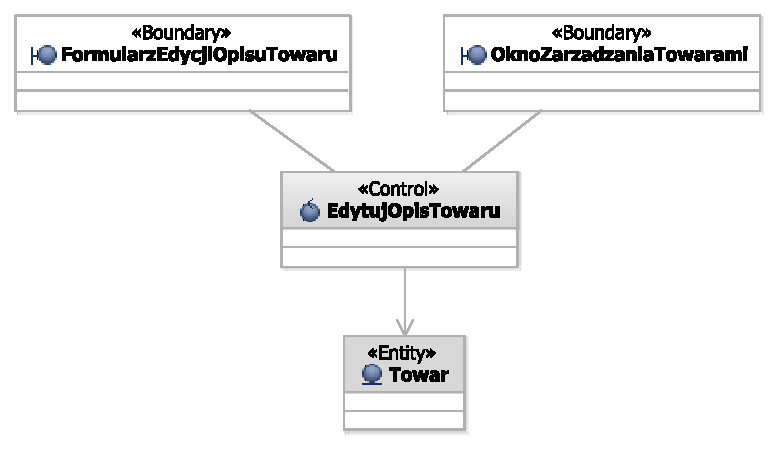
\includegraphics[angle=\ecbangle, scale=\ecbscale]{../img/usecase/pu20ecb.pdf}
  \caption{\ecbcaption20}
\end{figure}
\begin{figure}[H]
  \centering
  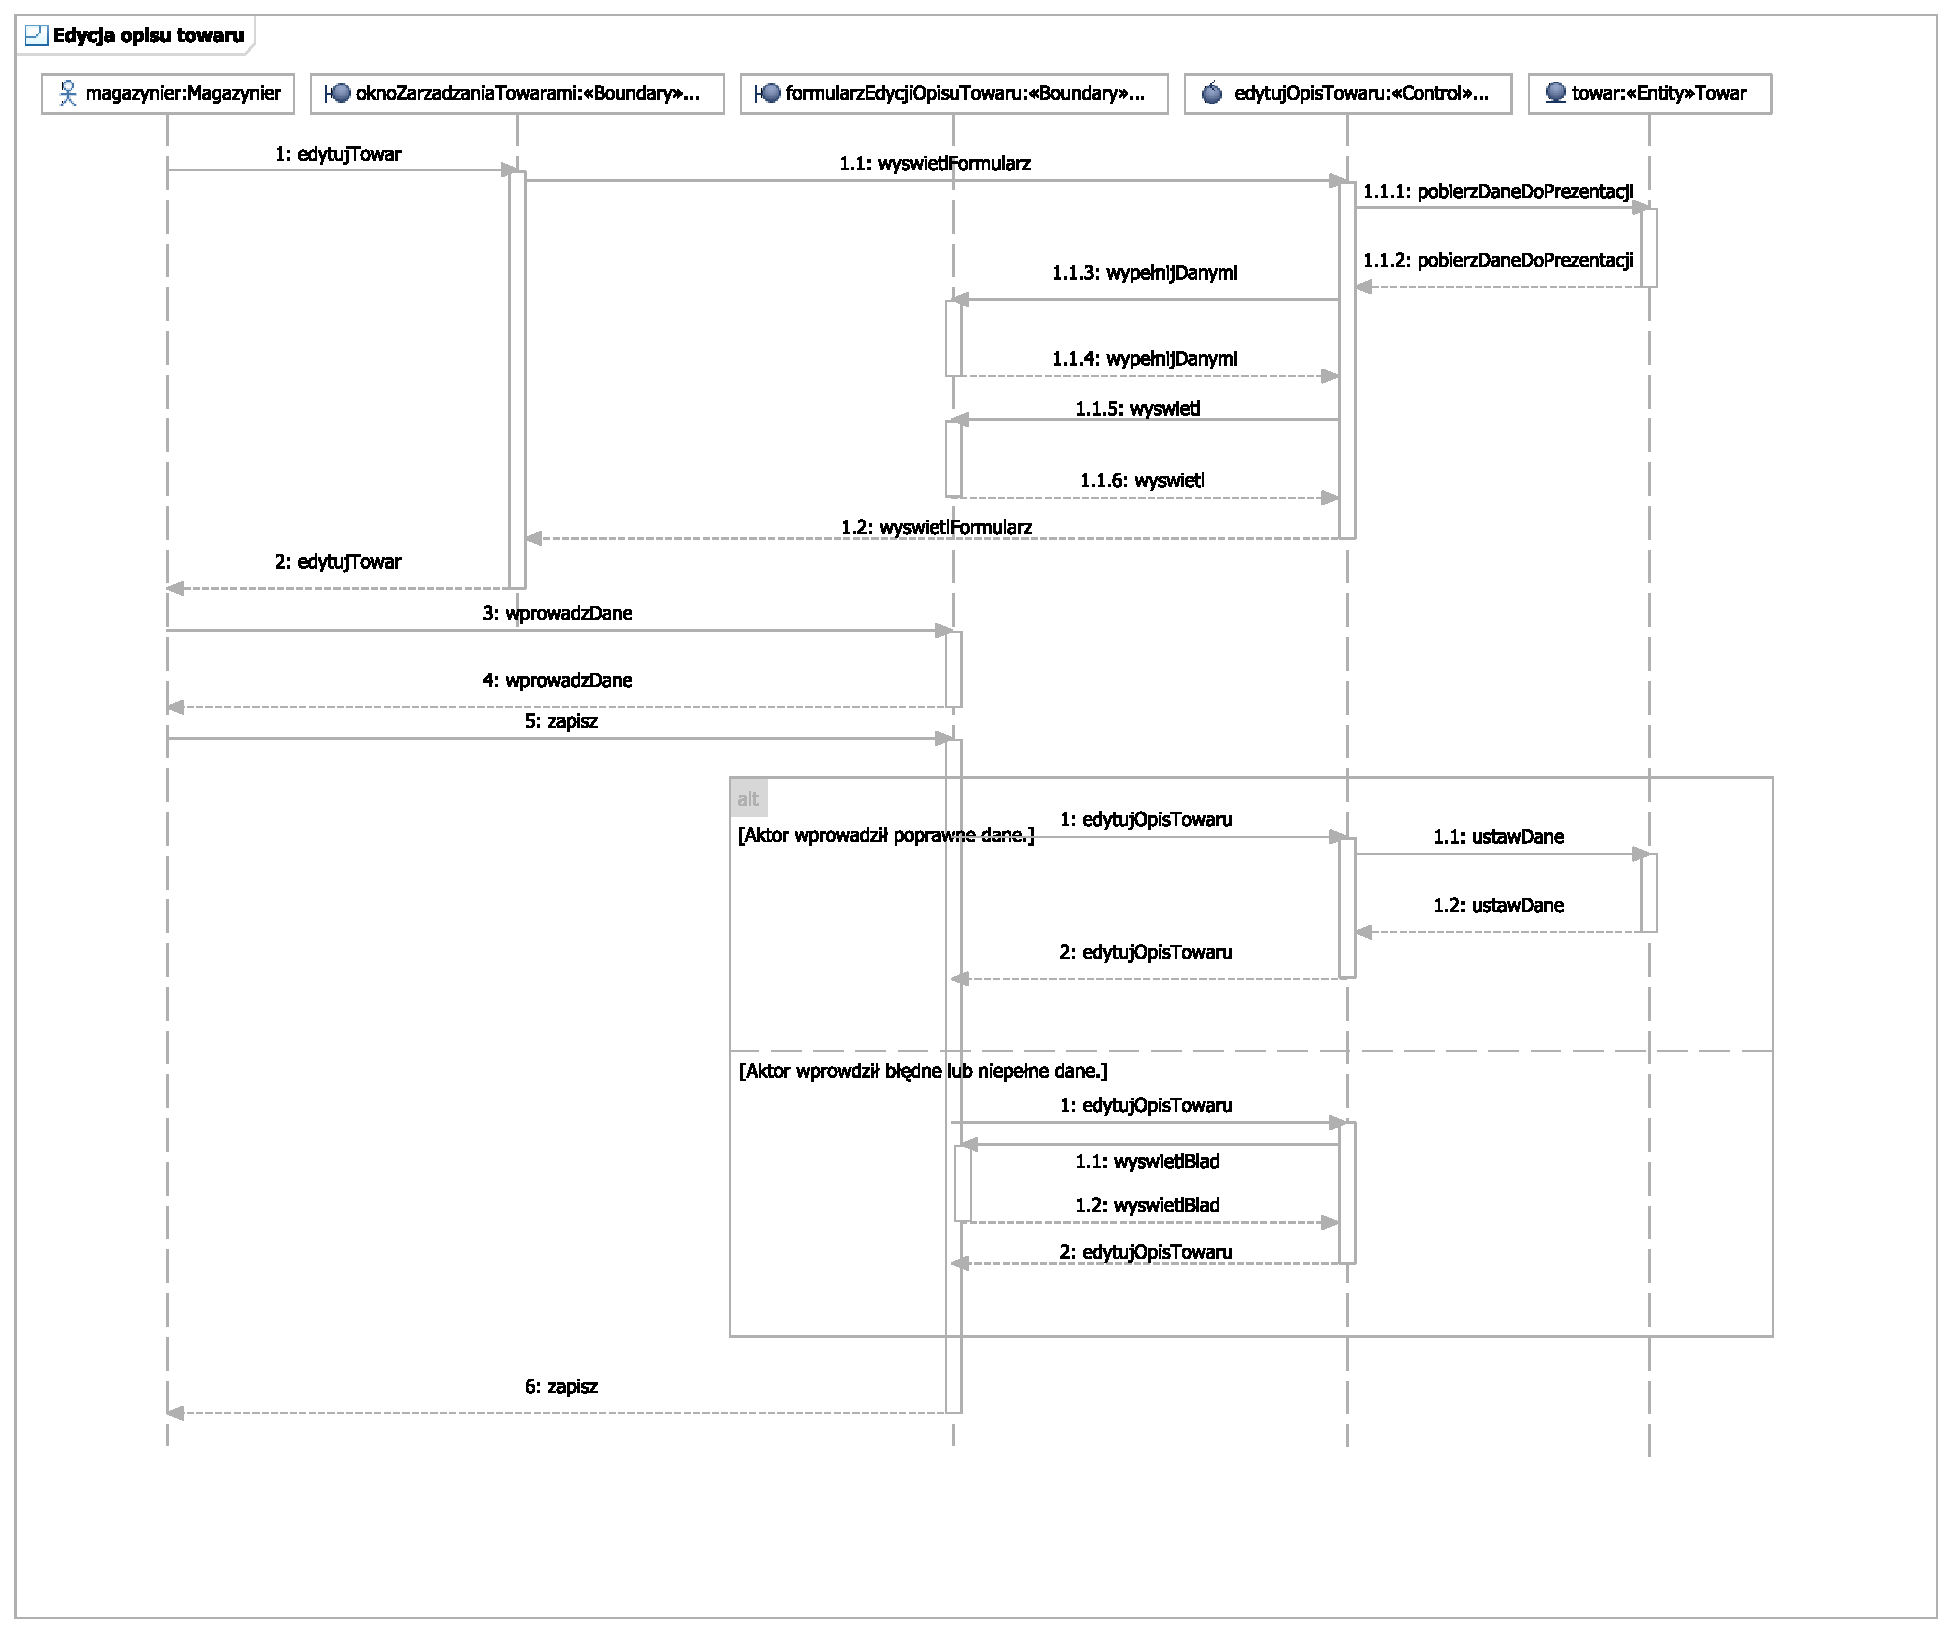
\includegraphics[angle=\seqangle, scale=0.45]{../img/usecase/pu20seq.pdf}
  \caption{\seqcaption20}
\end{figure}
\newpage

%%%%%%%
\subsection{Usuwanie danych towaru}
\begin{usecase}
  \addtitle{PU21}{Usuwanie danych towaru}
  \addfield{Priorytet:}{wysoki}
  \addfield{Aktor główny:}{Magazynier}
  \addfield{Rozszerza przypadki:}{PU18}
  \addfield{Warunki początkowe:}{Aktor został uwierzytelniony.}
  \additemizedfield{Warunki końcowe:}{
    \item Dane towaru zostały usunięte z systemu.
    \item Usunięty towar nie jest wypisywany na liście towarów w magazynie.
  }
  \addscenario{Scenariusz główny:}{
    \item Aktor wybiera opcję usunięcia danych towaru z systemu.
    \item System prosi o potwierdzenie operacji.
    \item Aktor potwierdza usunięcie towaru z systemu.
    \item System wyświetla informację o pomyślnym usunięciu towaru z systemu.
  }
  \addscenario{Scenariusz alternatywny:}{
    \item[4.a] Aktor anuluje usunięcie towaru z systemu.
      \begin{enumerate}
        \item[1.--2.] Jak w scenariuszu głównym.
        \item[3.] Aktor anuluje usunięcie towaru z systemu.
        \item[4.] System wyświetla informację, że operacja została anulowana.
      \end{enumerate}
  }
  \addfield{Wymagania funkcjonalne:}{2.3}
\end{usecase}

\begin{figure}[H]
  \centering
  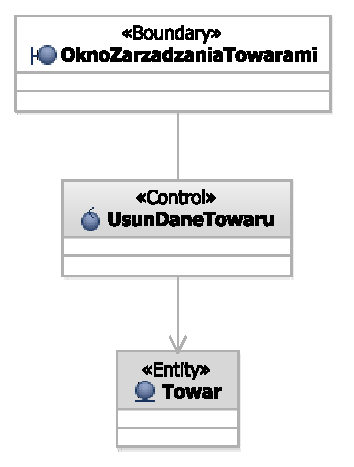
\includegraphics[angle=\ecbangle, scale=\ecbscale]{../img/usecase/pu21ecb.pdf}
  \caption{\ecbcaption21}
\end{figure}

\begin{figure}[H]
  \centering
  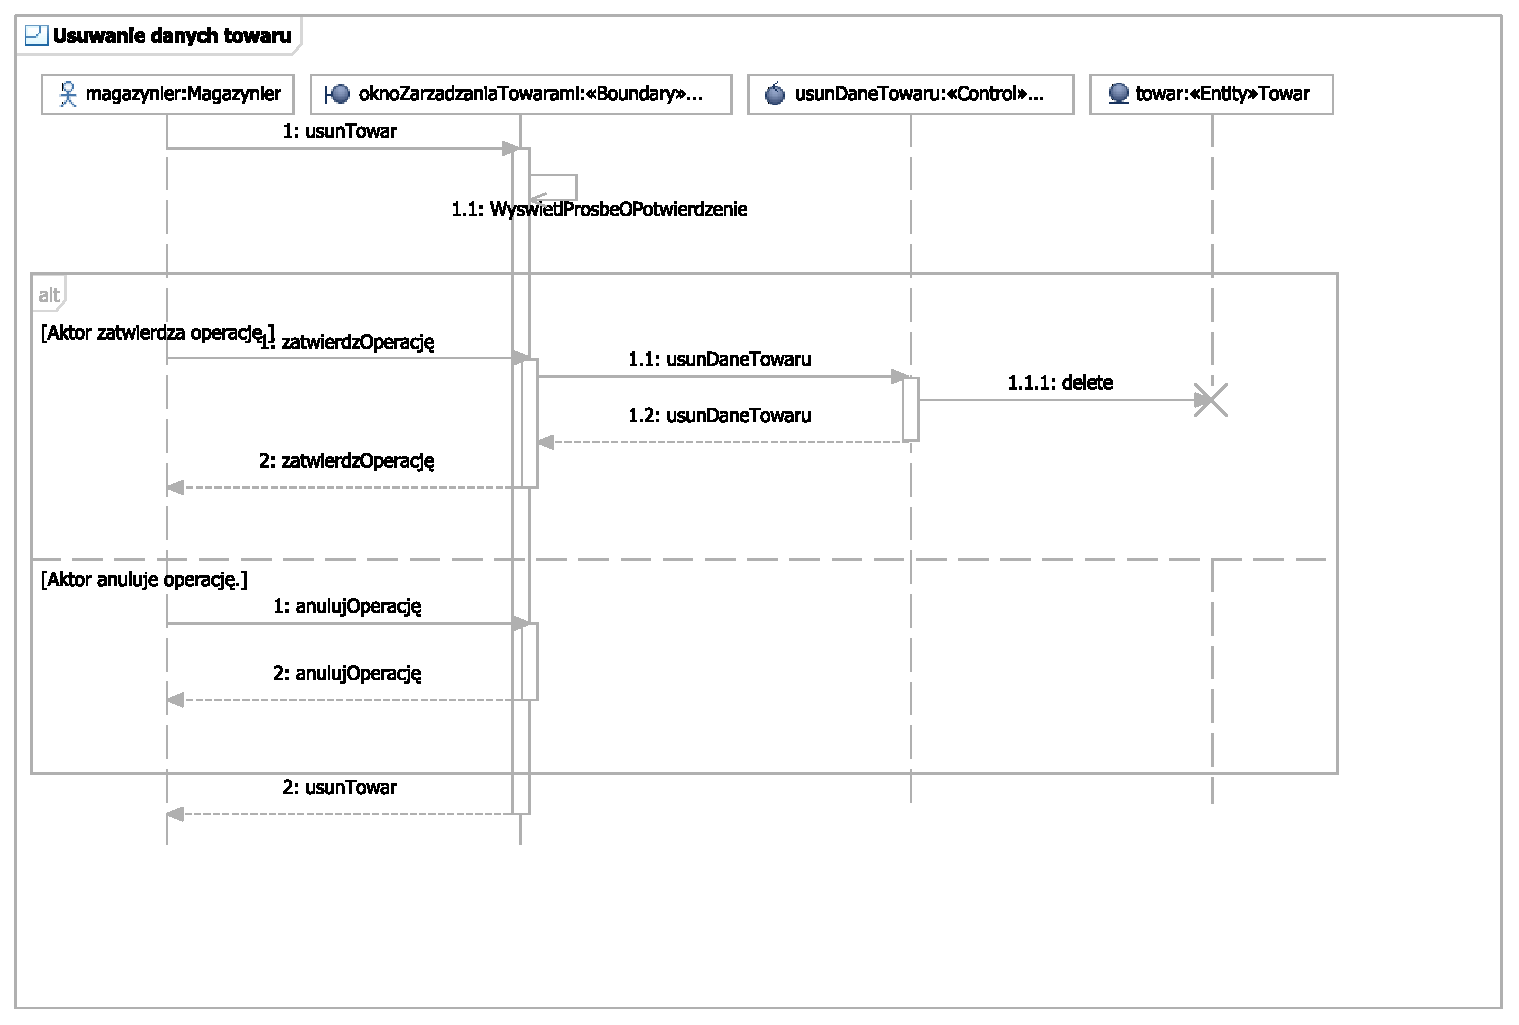
\includegraphics[angle=\seqangle, scale=\seqscale]{../img/usecase/pu21seq.pdf}
  \caption{\seqcaption21}
\end{figure}
\newpage

\subsection{Korekta stanu towaru}
\begin{usecase}
  \addtitle{PU22}{Korekta stanu towaru}
  \addfield{Priorytet:}{wysoki}
  \addfield{Aktor główny:}{Magazynier}
  \addfield{Rozszerza przypadki:}{PU18, PU20}
  \additemizedfield{Warunki początkowe:}{
    \item Aktor został uwierzytelniony.
    \item W systemie są zapisane dane co najmniej jednego towaru.
  }
  \additemizedfield{Warunki końcowe:} {
    \item Ilość towaru została zaktualizowana zgodnie z podaną wartością korekty oraz obecnym stanem towaru.
    \item Ilość towaru przechowywana w systemie musi spełniać warunki poprawności przedstawione w \ref{dziedzina-problemu}.
    \item W systemie został zapisany dokument korekty stanu towaru w magazynie.
  }
  \addscenario{Scenariusz główny:}{
     \item Aktor wybiera opcję utworzenia dokumentu korekty stanu towaru.
     \item System wyświetla formularz korekty stanu towaru.
     \item Aktor wypełnia podstawowe dane dokumentu.
     \item Aktor wybiera towary, których stan podlega korekcie w tworzonym dokumencie oraz podaje ich nowe ilości.
     \item Aktor wybiera opcję zapisania dokumentu.
     \item System informuje aktora, że dane zostały poprawnie zaktualizowane.
  }
  \addscenario{Scenariusz alternatywny:} {
     \item[3.a] Aktor podał niepoprawne dane.
       \begin{enumerate}
          \item[1--3.] Jak w scenariuszu głównym.
          \item[4.] System informuje aktora, że podana wartość nie jest prawidłowa.
          \item[5.] Aktor wraca do punktu 3.
       \end{enumerate}
     \item[4.a] Aktor wybrał ten sam towar co najmniej dwa razy.
       \begin{enumerate}
       \item[1--4.] Jak w scenariuszu głównym.
       \item[5.] System informuje aktora, że co najmniej dwa razy wybrał ten sam towar, podane ilości towaru zostaną więc zsumowane.
       \item[6.] System wyświetla zsumowane wartości dla tych samych towarów.
       \item[7--...] Jak w scenariuszu głównym.
       \end{enumerate}
  }
  \addfield{Zakres przetwarzanych danych:} {
    Dane wprowadzane zgodne z informacjami przedstawionymi w \ref{dziedzina-problemu}.
  }
  \addfield{Warunki poprawności danych:} {
    Takie jak przedstawione w \ref{dziedzina-problemu}.
  }
  \addfield{Wymagania funkcjonalne:}{2.2.2}
\end{usecase}

\begin{figure}[H]
  \centering
  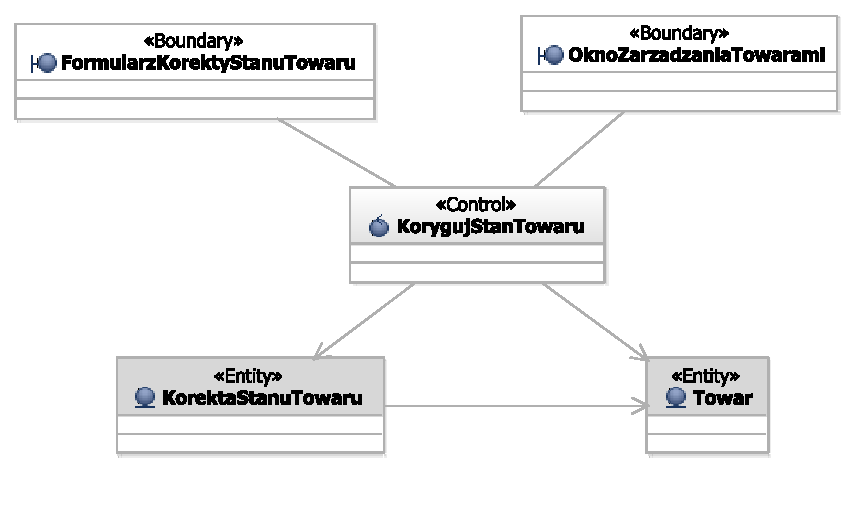
\includegraphics[angle=\ecbangle, scale=\ecbscale]{../img/usecase/pu22ecb.pdf}
  \caption{\ecbcaption22}
\end{figure}
\newpage
\begin{figure}[H]
  \centering
  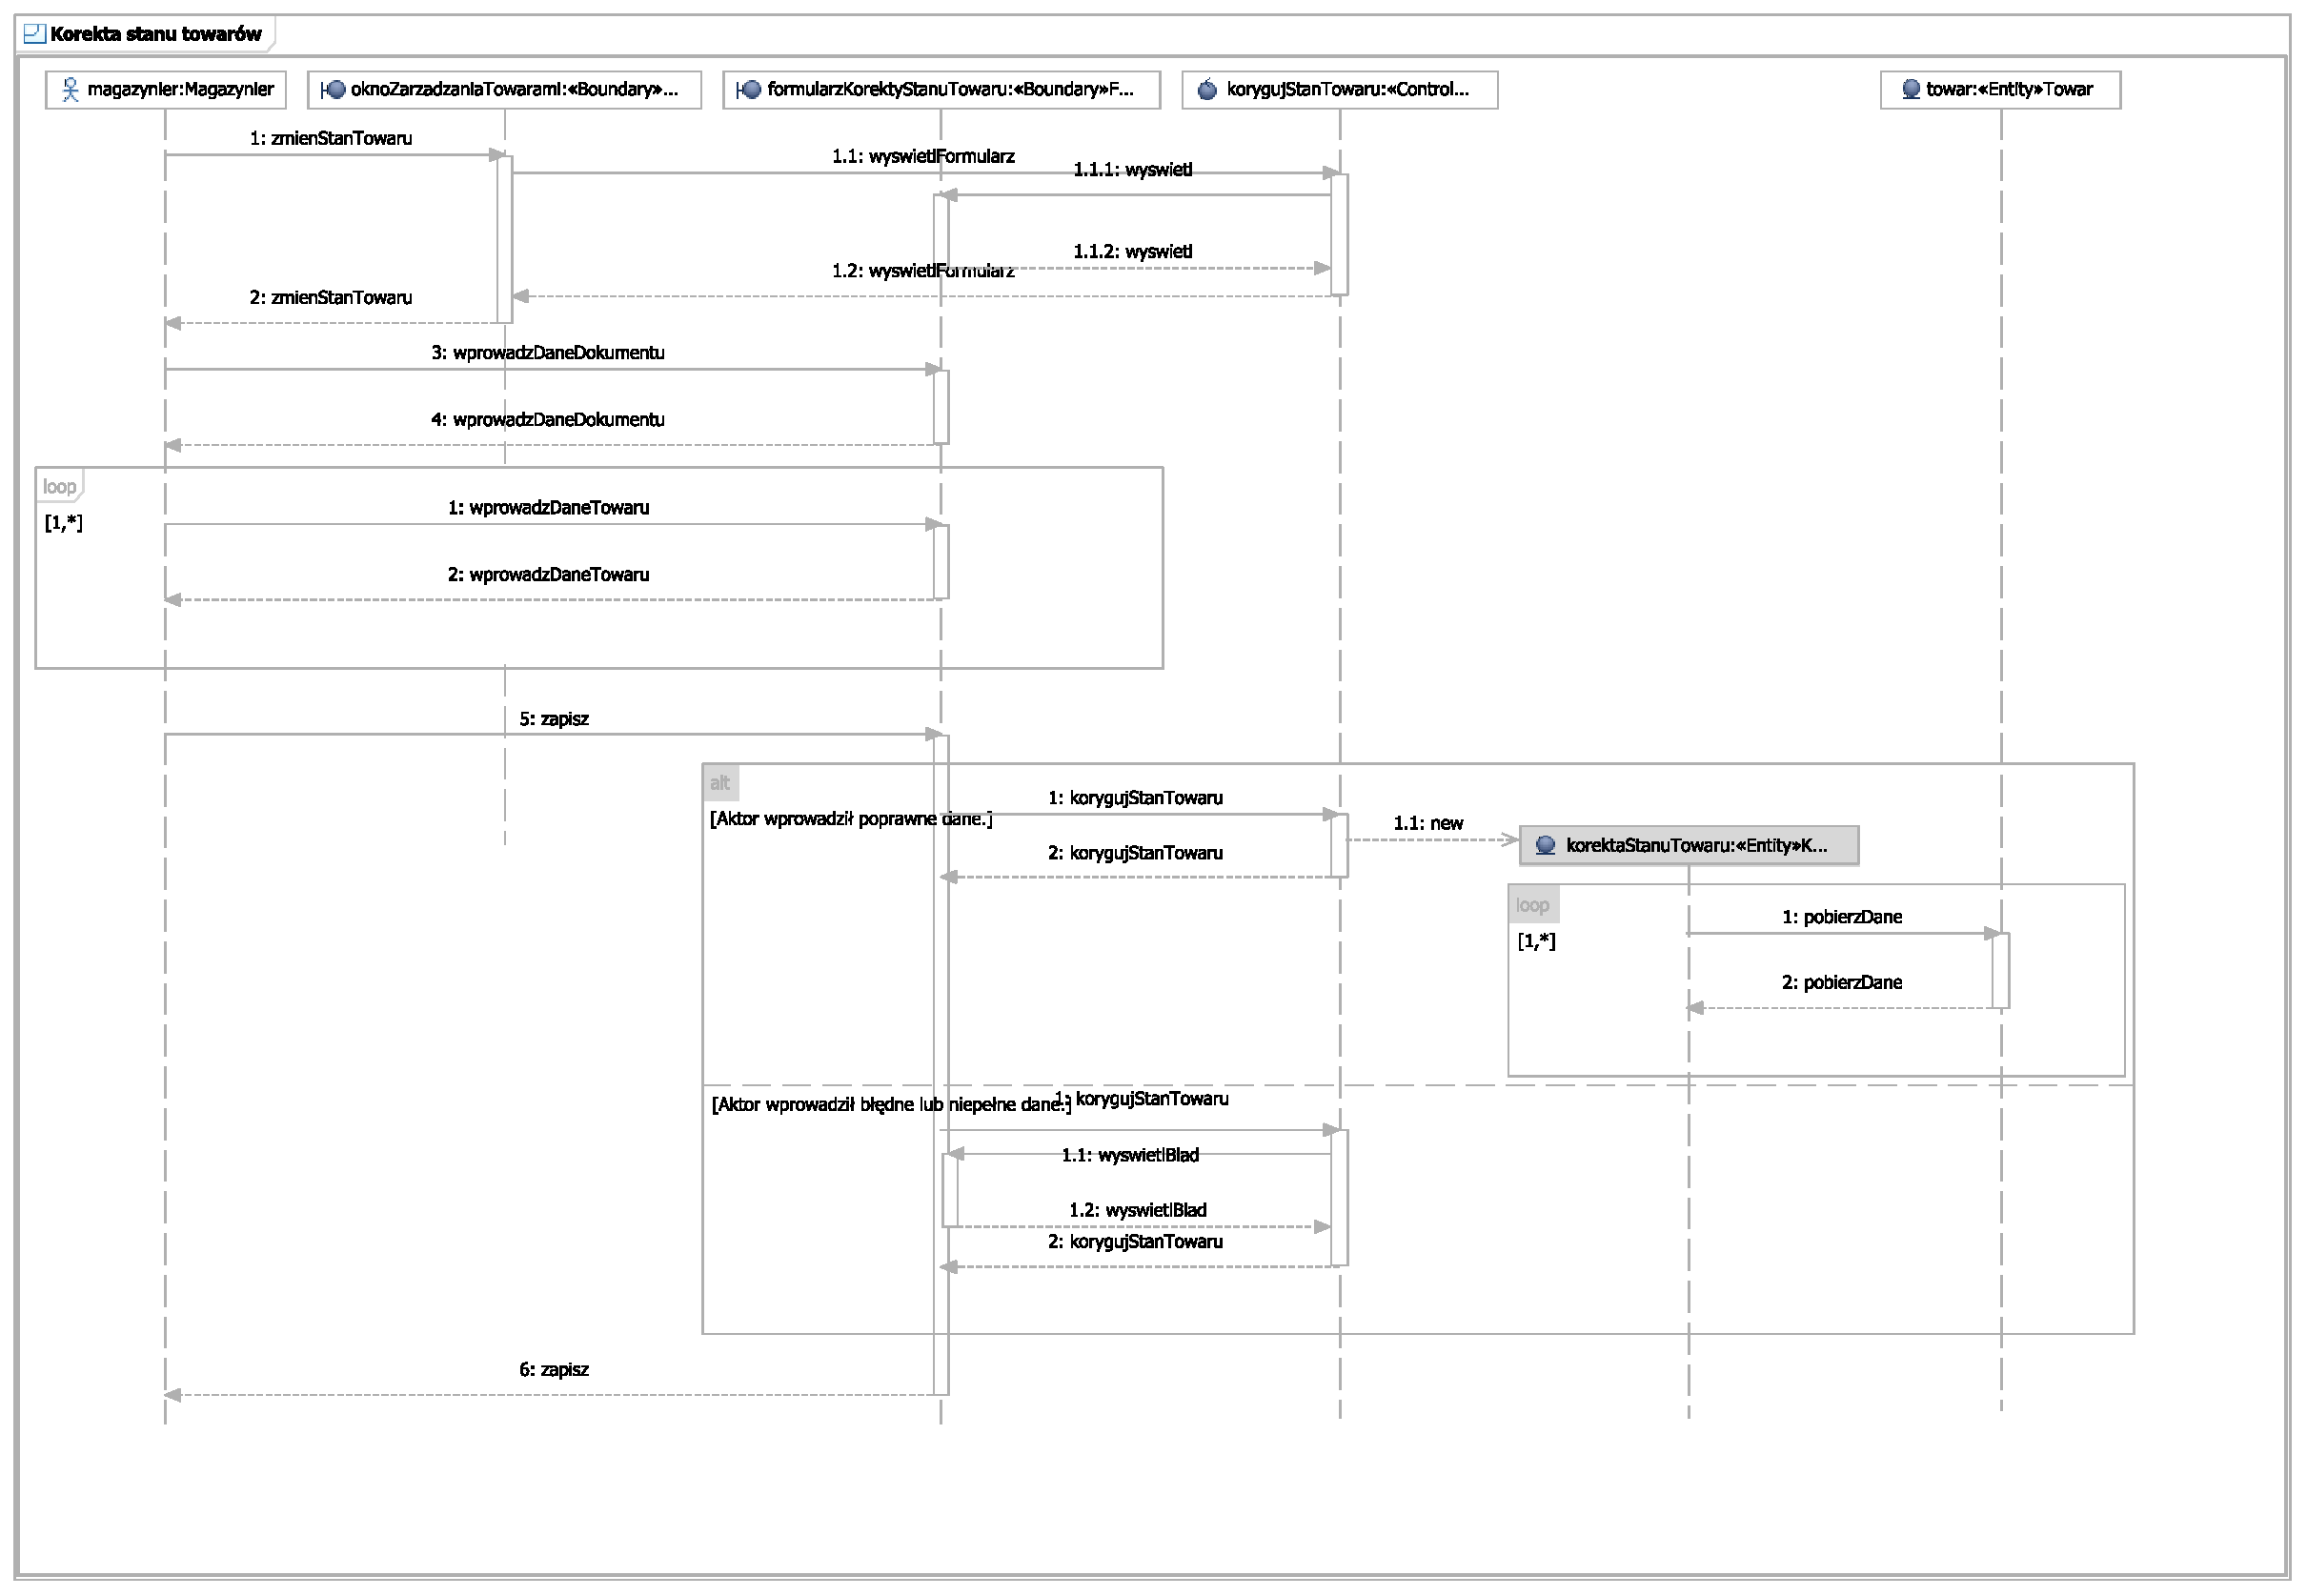
\includegraphics[angle=\seqangle, scale=0.40]{../img/usecase/pu22seq.pdf}
  \caption{\seqcaption22}
\end{figure}
\newpage

% %%%%%%
\subsection{Przyjęcie towaru na magazyn}
\begin{usecase}
  \addtitle{PU23}{Przyjęcie towaru na magazyn}
  \addfield{Priorytet:}{wysoki}
  \addfield{Aktor główny:}{Magazynier}
  \addfield{Warunki początkowe:}{Aktor został uwierzytelniony.}
  % Warunki końcowe (brak).
  \addscenario{Scenariusz główny:}{
  \item Aktor wybiera opcję przyjęcia towaru na magazyn.
  \item System wyświetla listę dokumentów PZ wraz z opcjami do zarządzania dokumentami przyjęcia towaru.
  }
  \addfield{Wymagania funkcjonalne:}{4.}
\end{usecase}

\begin{figure}[H]
  \centering
  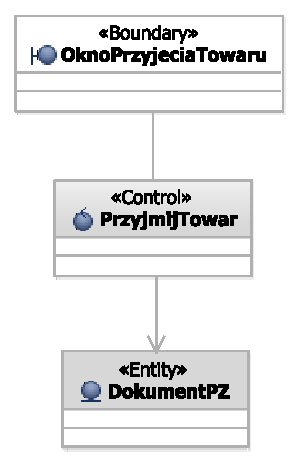
\includegraphics[angle=\ecbangle, scale=\ecbscale]{../img/usecase/pu23ecb.pdf}
  \caption{\ecbcaption23}
\end{figure}
\newpage
\begin{figure}[H]
  \centering
  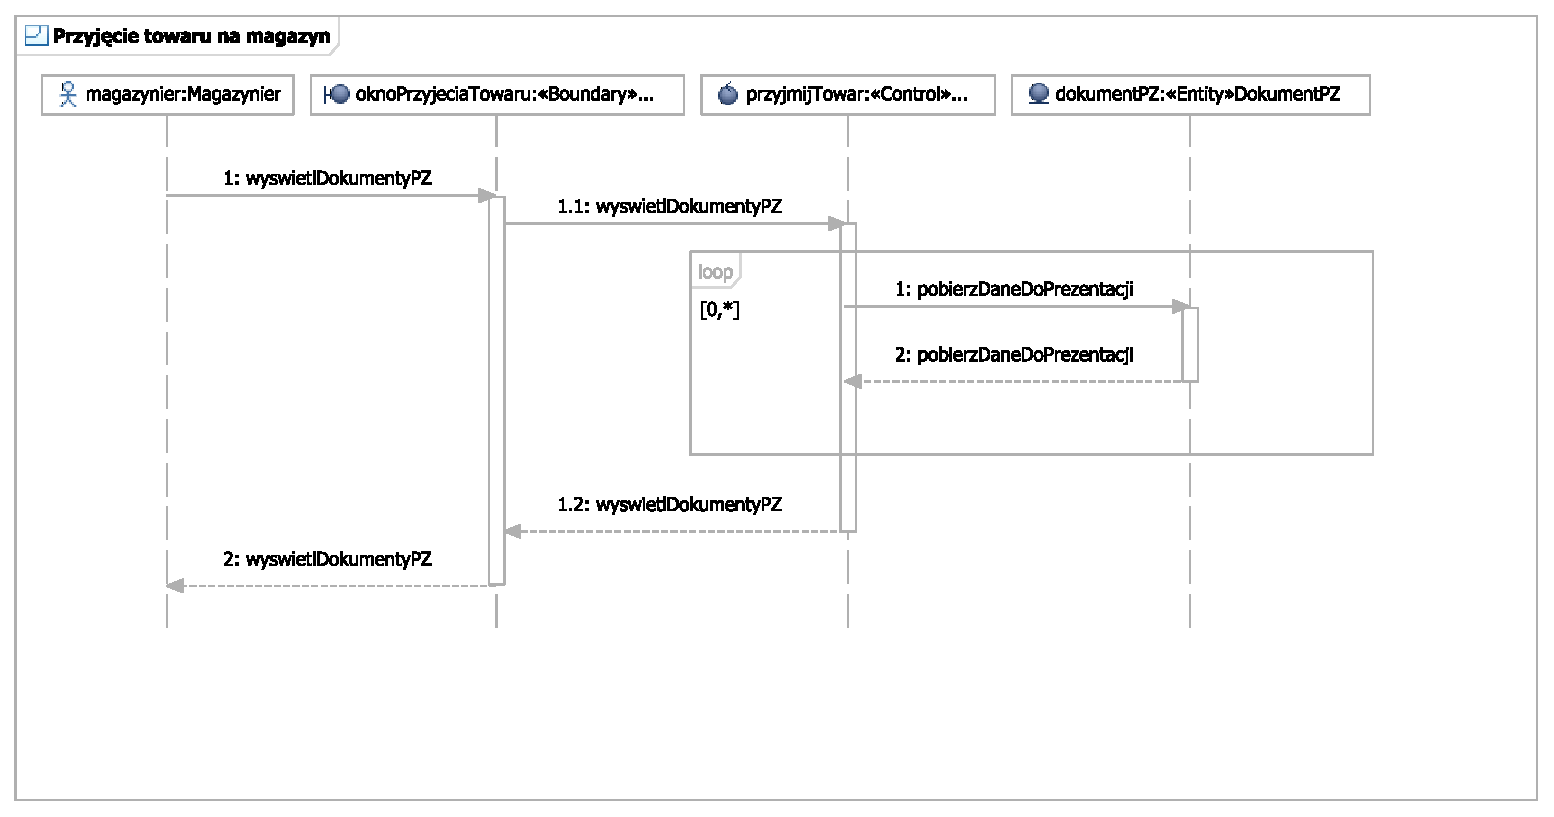
\includegraphics[angle=\seqangle, scale=\seqscale]{../img/usecase/pu23seq.pdf}
  \caption{\seqcaption23}
\end{figure}
\newpage

%%%%%%%
\subsection{Tworzenie dokumentu przyjęcia towaru}
\begin{usecase}
  \addtitle{PU24}{Tworzenie dokumentu przyjęcia towaru}
  \addfield{Priorytet:}{wysoki}
  \addfield{Aktor główny:}{Magazynier}
  \addfield{Rozszerza przypadki:}{PU23}
  \addfield{Warunki początkowe:}{Aktor został uwierzytelniony.}
  \additemizedfield{Warunki końcowe:}{ 
    \item Dokument przyjęcia towaru został zapisany w systemie.
    \item Aktor otrzymuje informacje o poprawnym dodaniu dokumentu do systemu.
    \item Użytkownik może wyświetlić dokument na liście dokumentów przyjęcia towaru. 
    \item Ilość przechowywanego towaru została zaktualizowana o ilość towaru zapisanego w dokumencie przyjęcia towaru.
    \item Ilość przechowywanego towaru jest zgodna z warunkami poprawności danych przedstawionymi w \ref{dziedzina-problemu}.
  }
  \addscenario{Scenariusz główny:}{
    \item Aktor wybiera opcję utworzenia nowego dokumentu przyjęcia towaru.
    \item System wyświetla formularz nowego dokumentu przyjęcia towaru.
    \item Aktor wypełnia podstawowe dane dokumentu.
    \item Aktor wybiera kontrahenta operacji.
    \item Aktor wybiera towary, które będą przyjęte od kontrahenta.
    \item Aktor wskazuje ilość oraz cenę jednostkową przyjmowanego towaru.
    \item Aktor wybiera opcję zapisania dokumentu.
    \item System informuje aktora, że dane zostały poprawnie zaktualizowane.
  }
  \addscenario{Scenariusz alternatywny:} {
    \item [3.a] Aktor nie podał wymaganych pól formularza:
      \begin{enumerate}
        \item[1--4.] Jak w scenariuszu głównym.
        \item[5.] System wyświetla powiadomienie o konieczności podania wymaganych informacji.
        \item[6.] Aktor wraca do punktu 3.  
      \end{enumerate}
    \item [3.b] Aktor podał błędne wartości pól formularza:
      \begin{enumerate}
        \item[1--4.] Jak w scenariuszu głównym.
        \item[5.] System wyświetla powiadomienie o błędnych polach formularza.
        \item[6.] Aktor wraca do punktu 3.
      \end{enumerate}
     \item[5.a] Aktor wybrał ten sam towar co najmniej dwa razy.
       \begin{enumerate}
       \item[1--5.] Jak w scenariuszu głównym.
       \item[6.] System informuje aktora, że co najmniej dwa razy wybrał ten sam towar, podane ilości towaru zostaną więc zsumowane.
       \item[7.] System wyświetla zsumowane wartości dla tych samych towarów.
       \item[8--...] Jak w scenariuszu głównym.
       \end{enumerate}
  }
  \addfield{Zakres przetwarzanych danych:} {
    Pola dokumentu przyjęcia towaru takie jak przedstawione w rozdziale \ref{dziedzina-problemu}.
  }
  \addfield{Warunki poprawności danych:}{
    Warunki poprawności takie jak przedstawione w rozdziale \ref{dziedzina-problemu}.
  }
  \addfield{Wymagania funkcjonalne:}{4.1}
\end{usecase}

\begin{figure}[H]
  \centering
  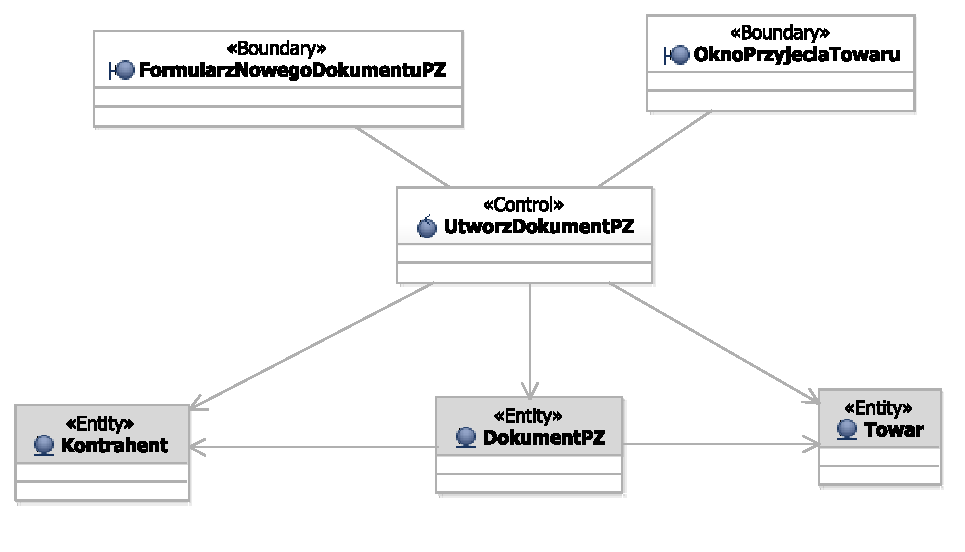
\includegraphics[angle=\ecbangle, scale=\ecbscale]{../img/usecase/pu24ecb.pdf}
  \caption{\ecbcaption24}
\end{figure}
\newpage
\begin{figure}[H]
  \centering
  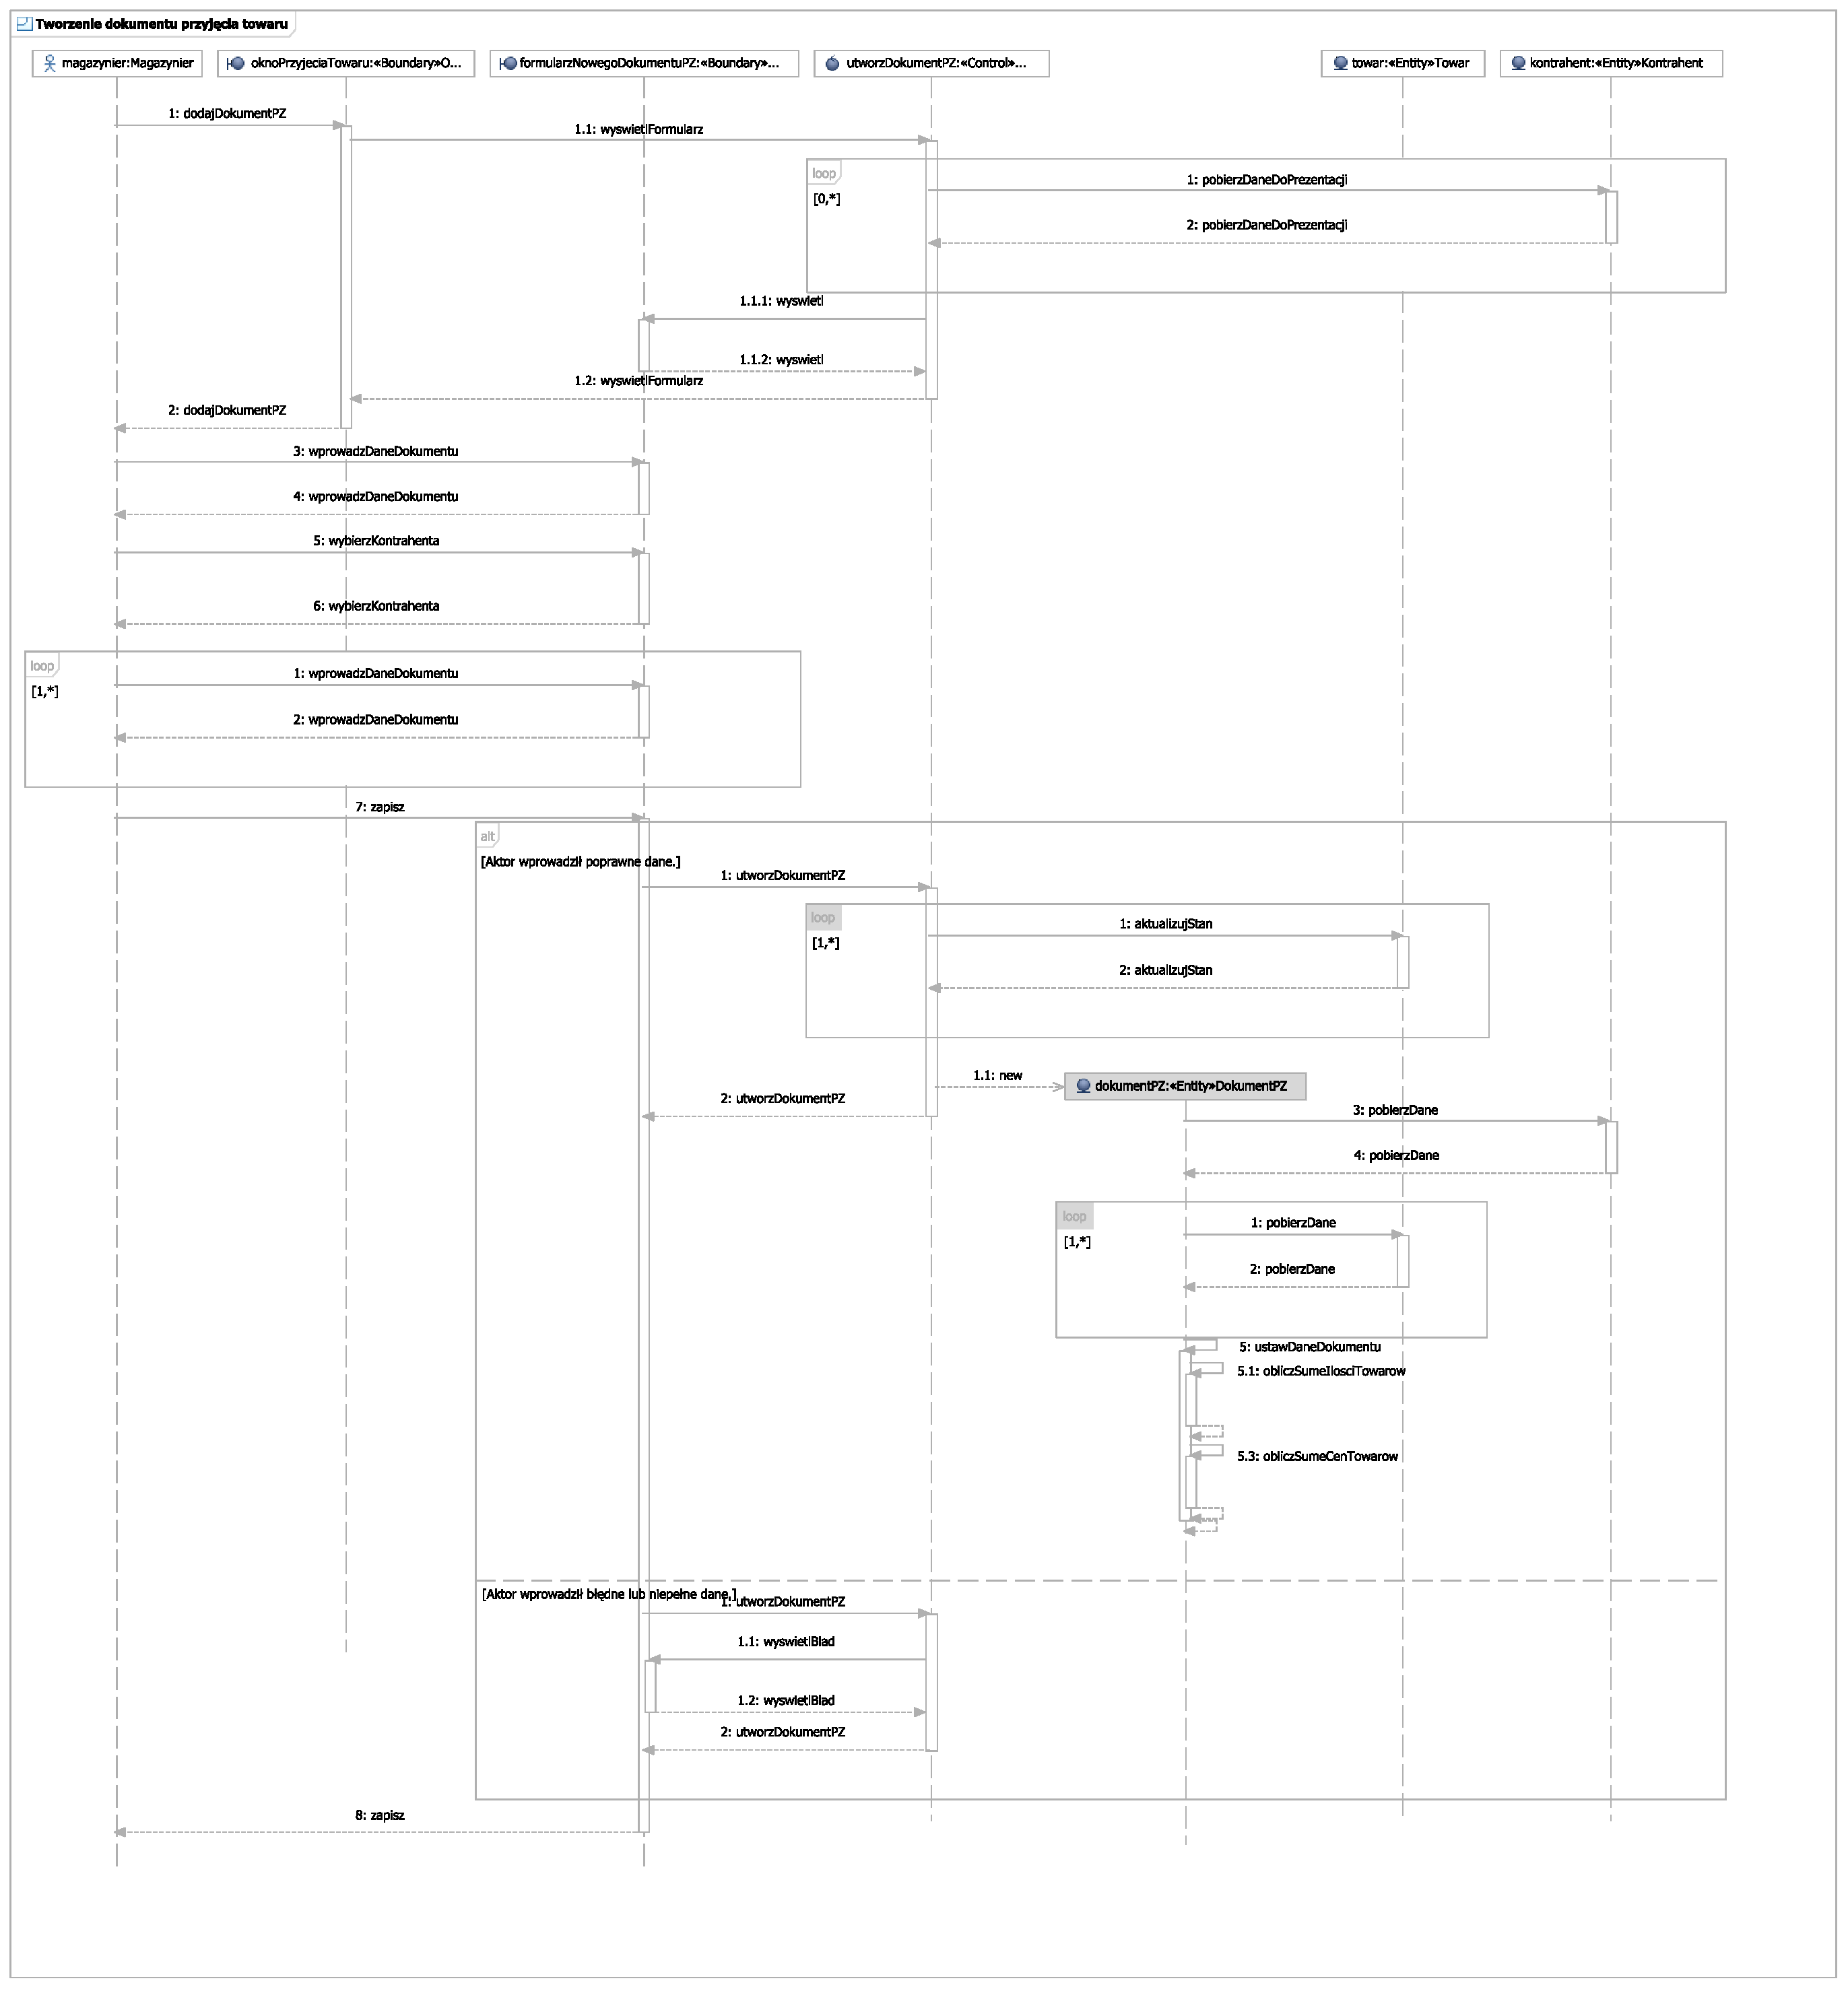
\includegraphics[angle=\seqangle, scale=0.35]{../img/usecase/pu24seq.pdf}
  \caption{\seqcaption24}
\end{figure}
\newpage

%%%%%%%%
\subsection{Edycja dokumentu przyjęcia towaru}
\begin{usecase}
  \addtitle{PU25}{Edycja dokumentu przyjęcia towaru}
  \addfield{Priorytet:}{wysoki}
  \addfield{Aktor główny:}{Magazynier}
  \addfield{Rozszerza przypadki:}{PU23}
  \additemizedfield{Warunki początkowe:}{
    \item Aktor został uwierzytelniony.
    \item Operacja przyjęcia towaru, którego dotyczy wybrany dokument, nie została jeszcze zrealizowana.
  }
  \additemizedfield{Warunki końcowe:}{ 
    \item Dane dokumentu zostały zaktualizowane w systemie.
    \item Użytkownik może wyświetlić dane dokumentu na liście dokumentów przyjęcia towaru. 
    \item Ilość przechowywanego towaru została zaktualizowana o ilość towaru zapisanego w dokumencie przyjęcia towaru.
    \item Ilość przechowywanego towaru jest zgodna z warunkami poprawności danych przedstawionymi w \ref{dziedzina-problemu}.
  }
  % TODO prawie duplikacja z Tworzeniem dokumentu przyjęcia towaru
  \addscenario{Scenariusz główny:}{
    \item Aktor wybiera opcję edycji wybranego dokumentu przyjęcia towaru.
    \item System wyświetla formularz edycji dokumentu przyjęcia towaru.
    \item Aktor wypełnia podstawowe dane dokumentu (oprócz pól wykluczonych z edycji).
    \item Aktor aktualizuje listę towarów, ich ilości oraz ceny jednostkowe.
    \item Aktor wybiera opcję aktualizacji dokumentu.
    \item System informuje aktora, że dane zostały poprawnie zaktualizowane.
  }
  \addscenario{Scenariusz alternatywny:} {
    \item [3.a] Aktor nie podał wymaganych pól formularza:
      \begin{enumerate}
        \item[1--4.] Jak w scenariuszu głównym.
        \item[5.] System wyświetla powiadomienie o konieczności podania wymaganych informacji.
        \item[6.] Aktor wraca do punktu 3.  
      \end{enumerate}
    \item [3.b] Aktor podał błędne wartości pól formularza:
      \begin{enumerate}
        \item[1--4.] Jak w scenariuszu głównym.
        \item[5.] System wyświetla powiadomienie o błędnych polach formularza.
        \item[6.] Aktor wraca do punktu 3.
      \end{enumerate}
     \item[4.a] Aktor wybrał ten sam towar co najmniej dwa razy.
       \begin{enumerate}
       \item[1--4.] Jak w scenariuszu głównym.
       \item[5.] System informuje aktora, że co najmniej dwa razy wybrał ten sam towar, podane ilości towaru zostaną więc zsumowane.
       \item[6.] System wyświetla zsumowane wartości dla tych samych towarów.
       \item[7--...] Jak w scenariuszu głównym.
       \end{enumerate}
  }
  \addfield{Zakres przetwarzanych danych:} {
    Pola dokumentu przyjęcia towaru takie jak przedstawione w rozdziale \ref{dziedzina-problemu}.
  }
  \addfield{Warunki poprawności danych:}{
    Warunki poprawności takie jak przedstawione w rozdziale \ref{dziedzina-problemu}.
  }
  \addfield{Wymagania funkcjonalne:}{4.2}
\end{usecase}

\begin{figure}[H]
  \centering
  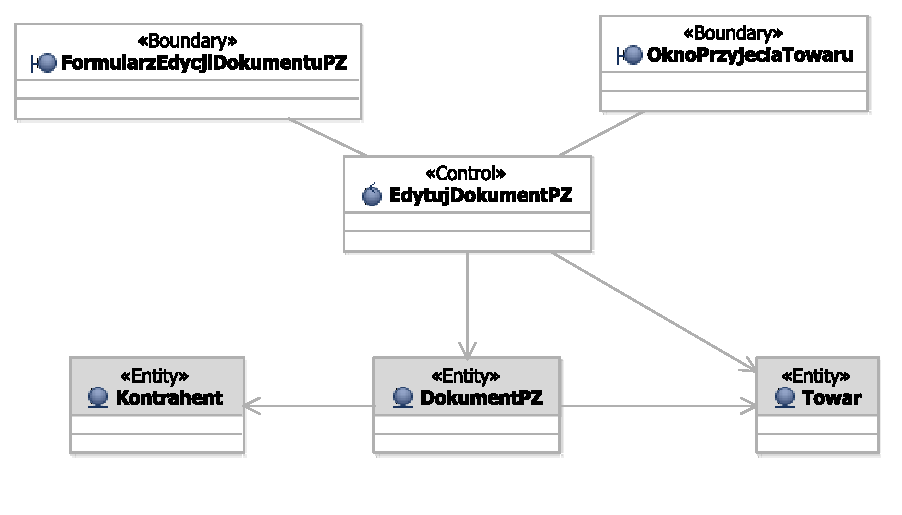
\includegraphics[angle=\ecbangle, scale=\ecbscale]{../img/usecase/pu25ecb.pdf}
  \caption{\ecbcaption25}
\end{figure}
\newpage
\begin{figure}[H]
  \centering
  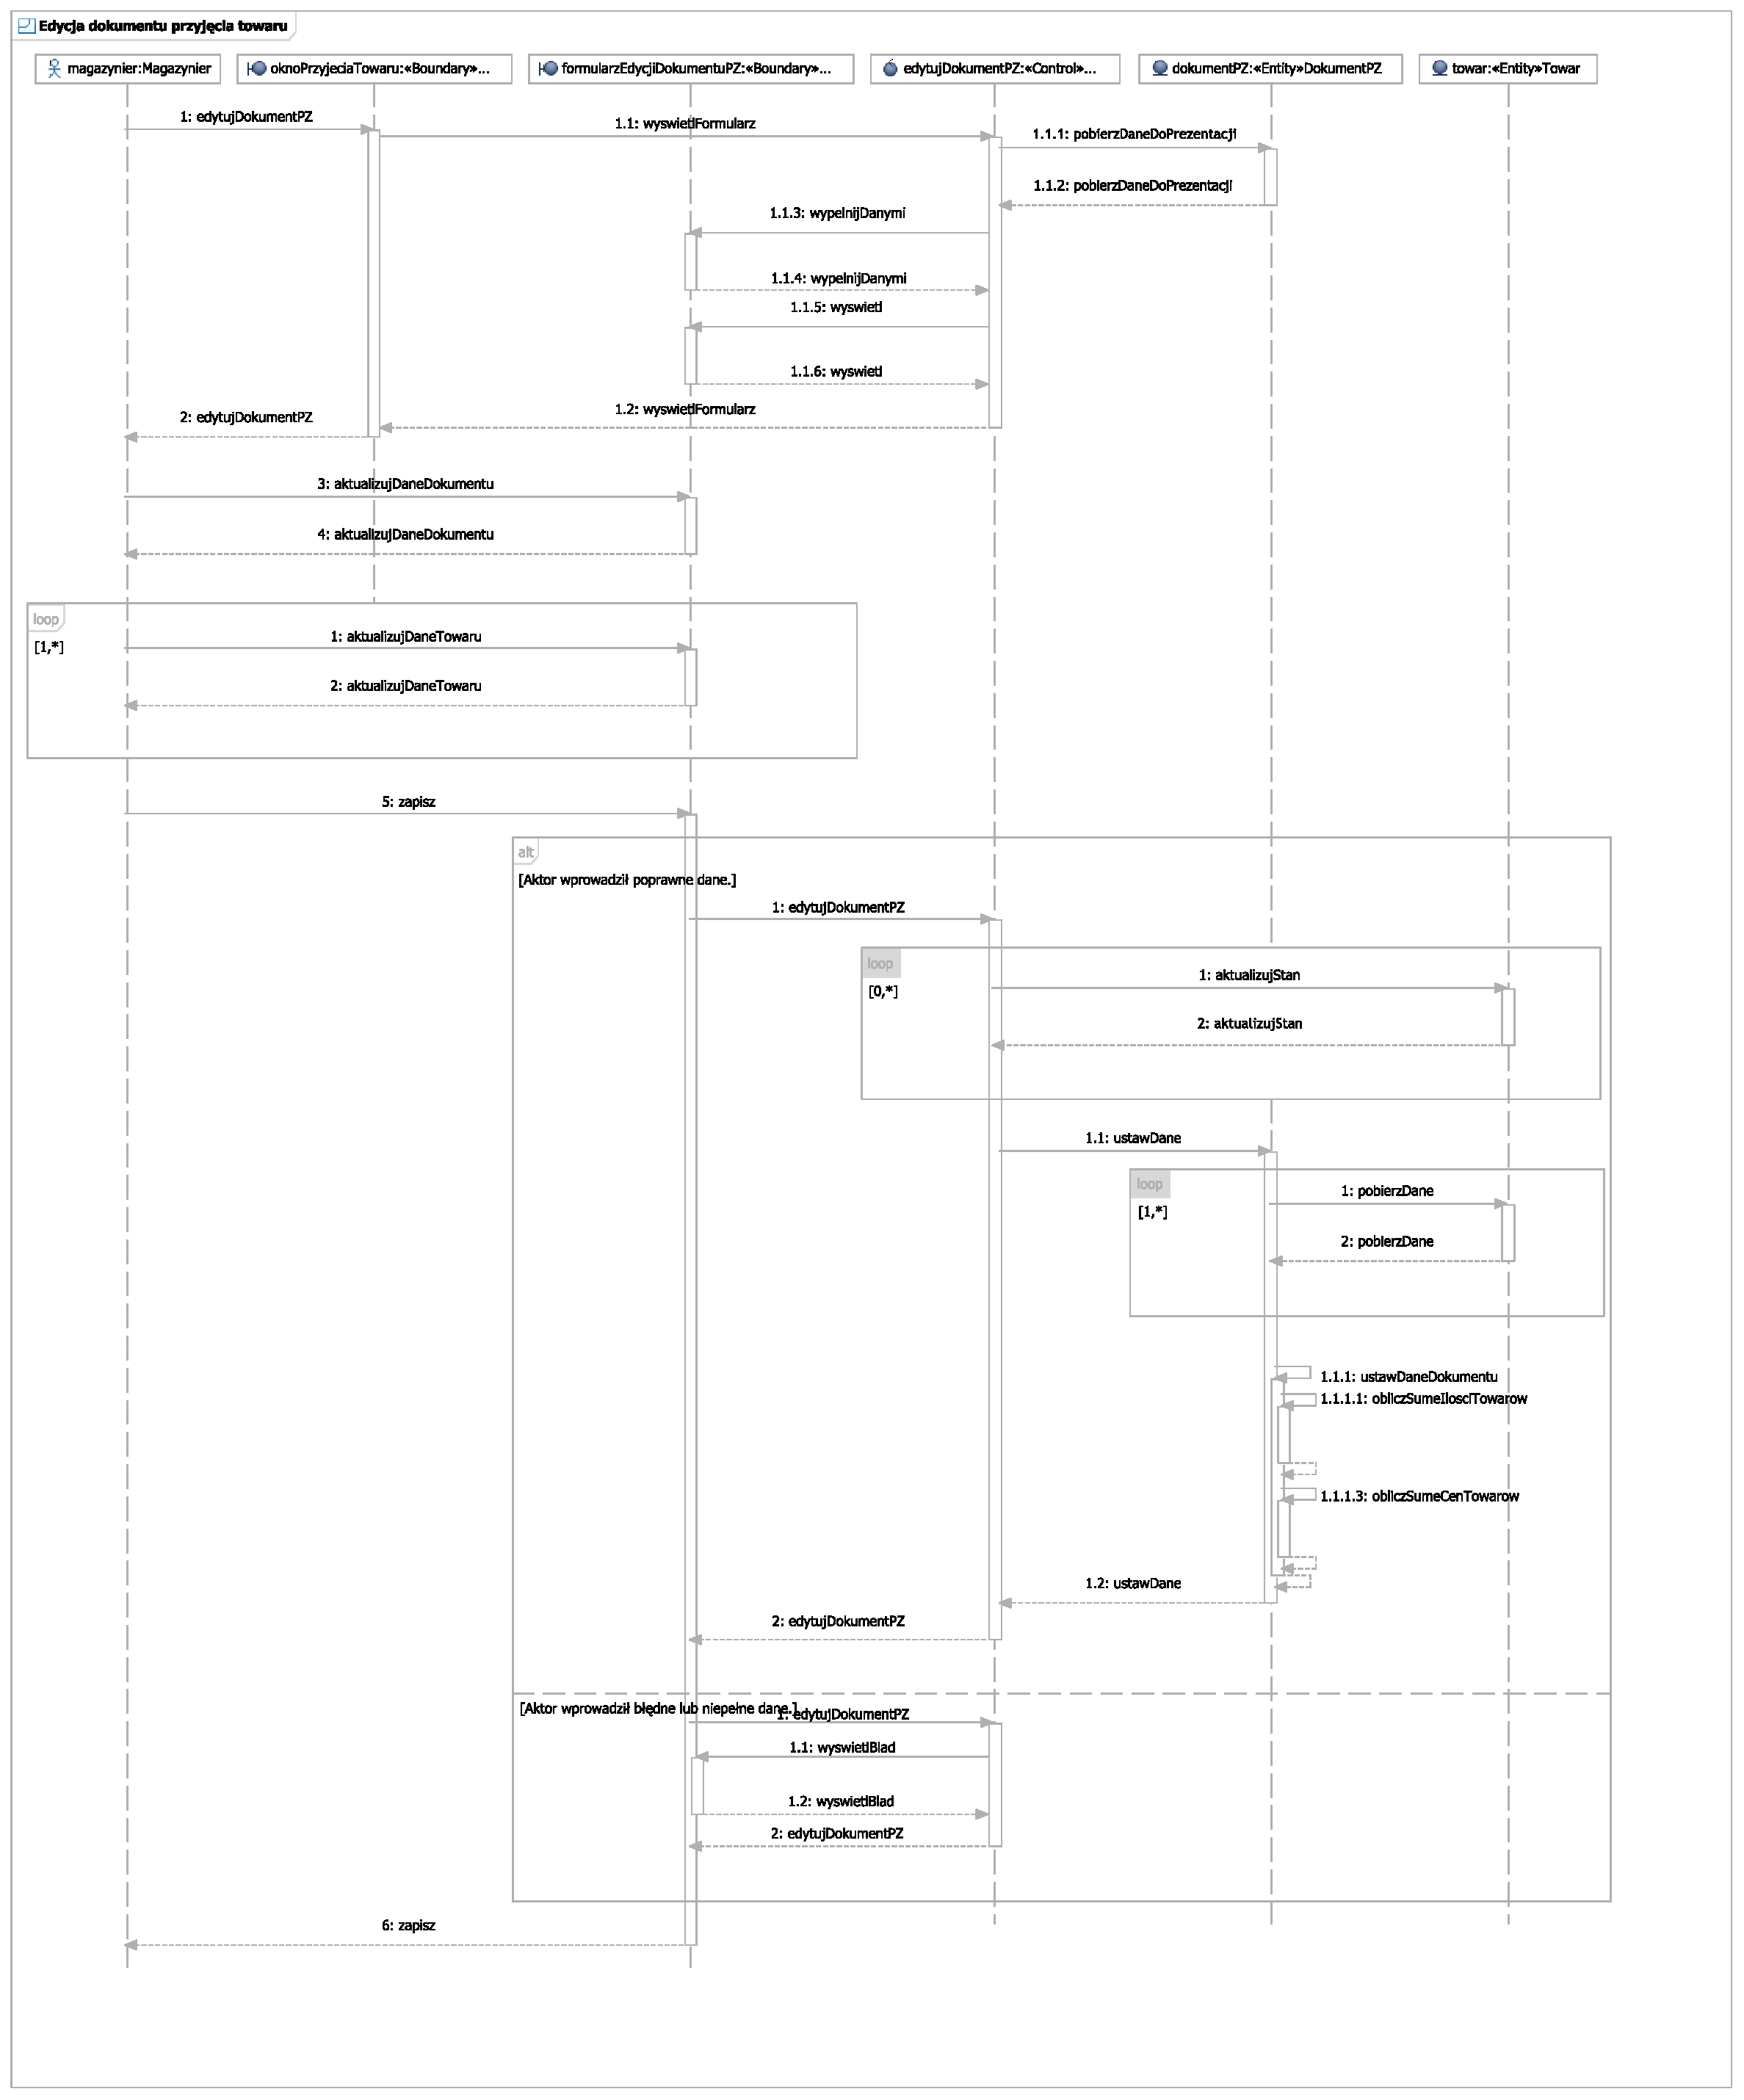
\includegraphics[angle=\seqangle, scale=\seqscalemin]{../img/usecase/pu25seq.pdf}
  \caption{\seqcaption25}
\end{figure}
\newpage

\subsection{Usuwanie dokumentu przyjęcia towaru}
\begin{usecase}
  \addtitle{PU26}{Usuwanie dokumentu przyjęcia towaru}
  \addfield{Priorytet:}{wysoki}
  \addfield{Aktor główny:}{Magazynier}
  \addfield{Rozszerza przypadki:}{PU23}
  \addfield{Warunki początkowe:}{Aktor został uwierzytelniony.}
  \additemizedfield{Warunki końcowe:}{
    \item Dane dokumentu zostały usunięte z systemu.
    \item Usunięty dokument nie jest wypisywany na liście dokumentów przyjęcia towaru.
    \item Stan towarów z usuniętego dokumentu jest zaktualizowany o ilości zapisane w usuwanym dokumencie.
  }
  \addscenario{Scenariusz główny:}{
    \item Aktor wybiera opcję usunięcia dokumentu przyjęcia towaru z systemu.
    \item System prosi o potwierdzenie operacji.
    \item Aktor potwierdza usunięcie dokumentu z systemu.
    \item System wyświetla informację o pomyślnym usunięciu dokumentu z systemu.
  }
  \addscenario{Scenariusz alternatywny:}{
    \item[2.a] Aktor anuluje usunięcie dokumentu z systemu.
      \begin{enumerate}
        \item[1.--2.] Jak w scenariuszu głównym.
        \item[3.] Aktor anuluje usunięcie dokumentu z systemu.
        \item[4.] System wyświetla informację, że operacja została anulowana.
      \end{enumerate}
  }
  \addfield{Wymagania funkcjonalne:}{4.3}
\end{usecase}

\begin{figure}[H]
  \centering
  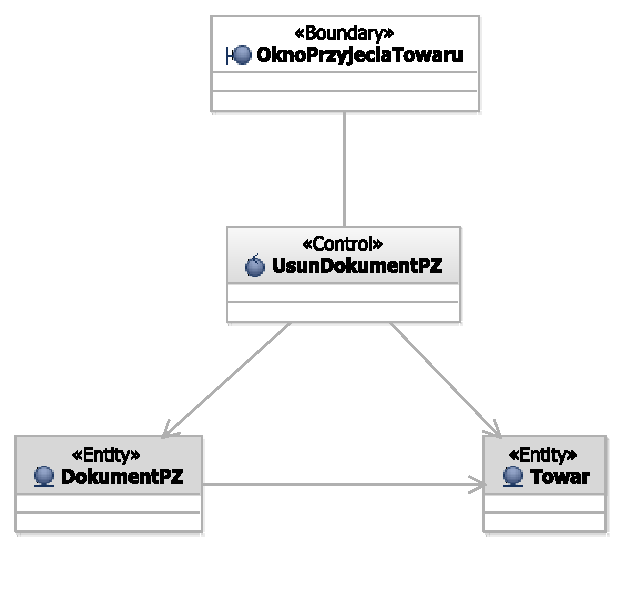
\includegraphics[angle=\ecbangle, scale=\ecbscale]{../img/usecase/pu26ecb.pdf}
  \caption{\ecbcaption26}
\end{figure}

\begin{figure}[H]
  \centering
  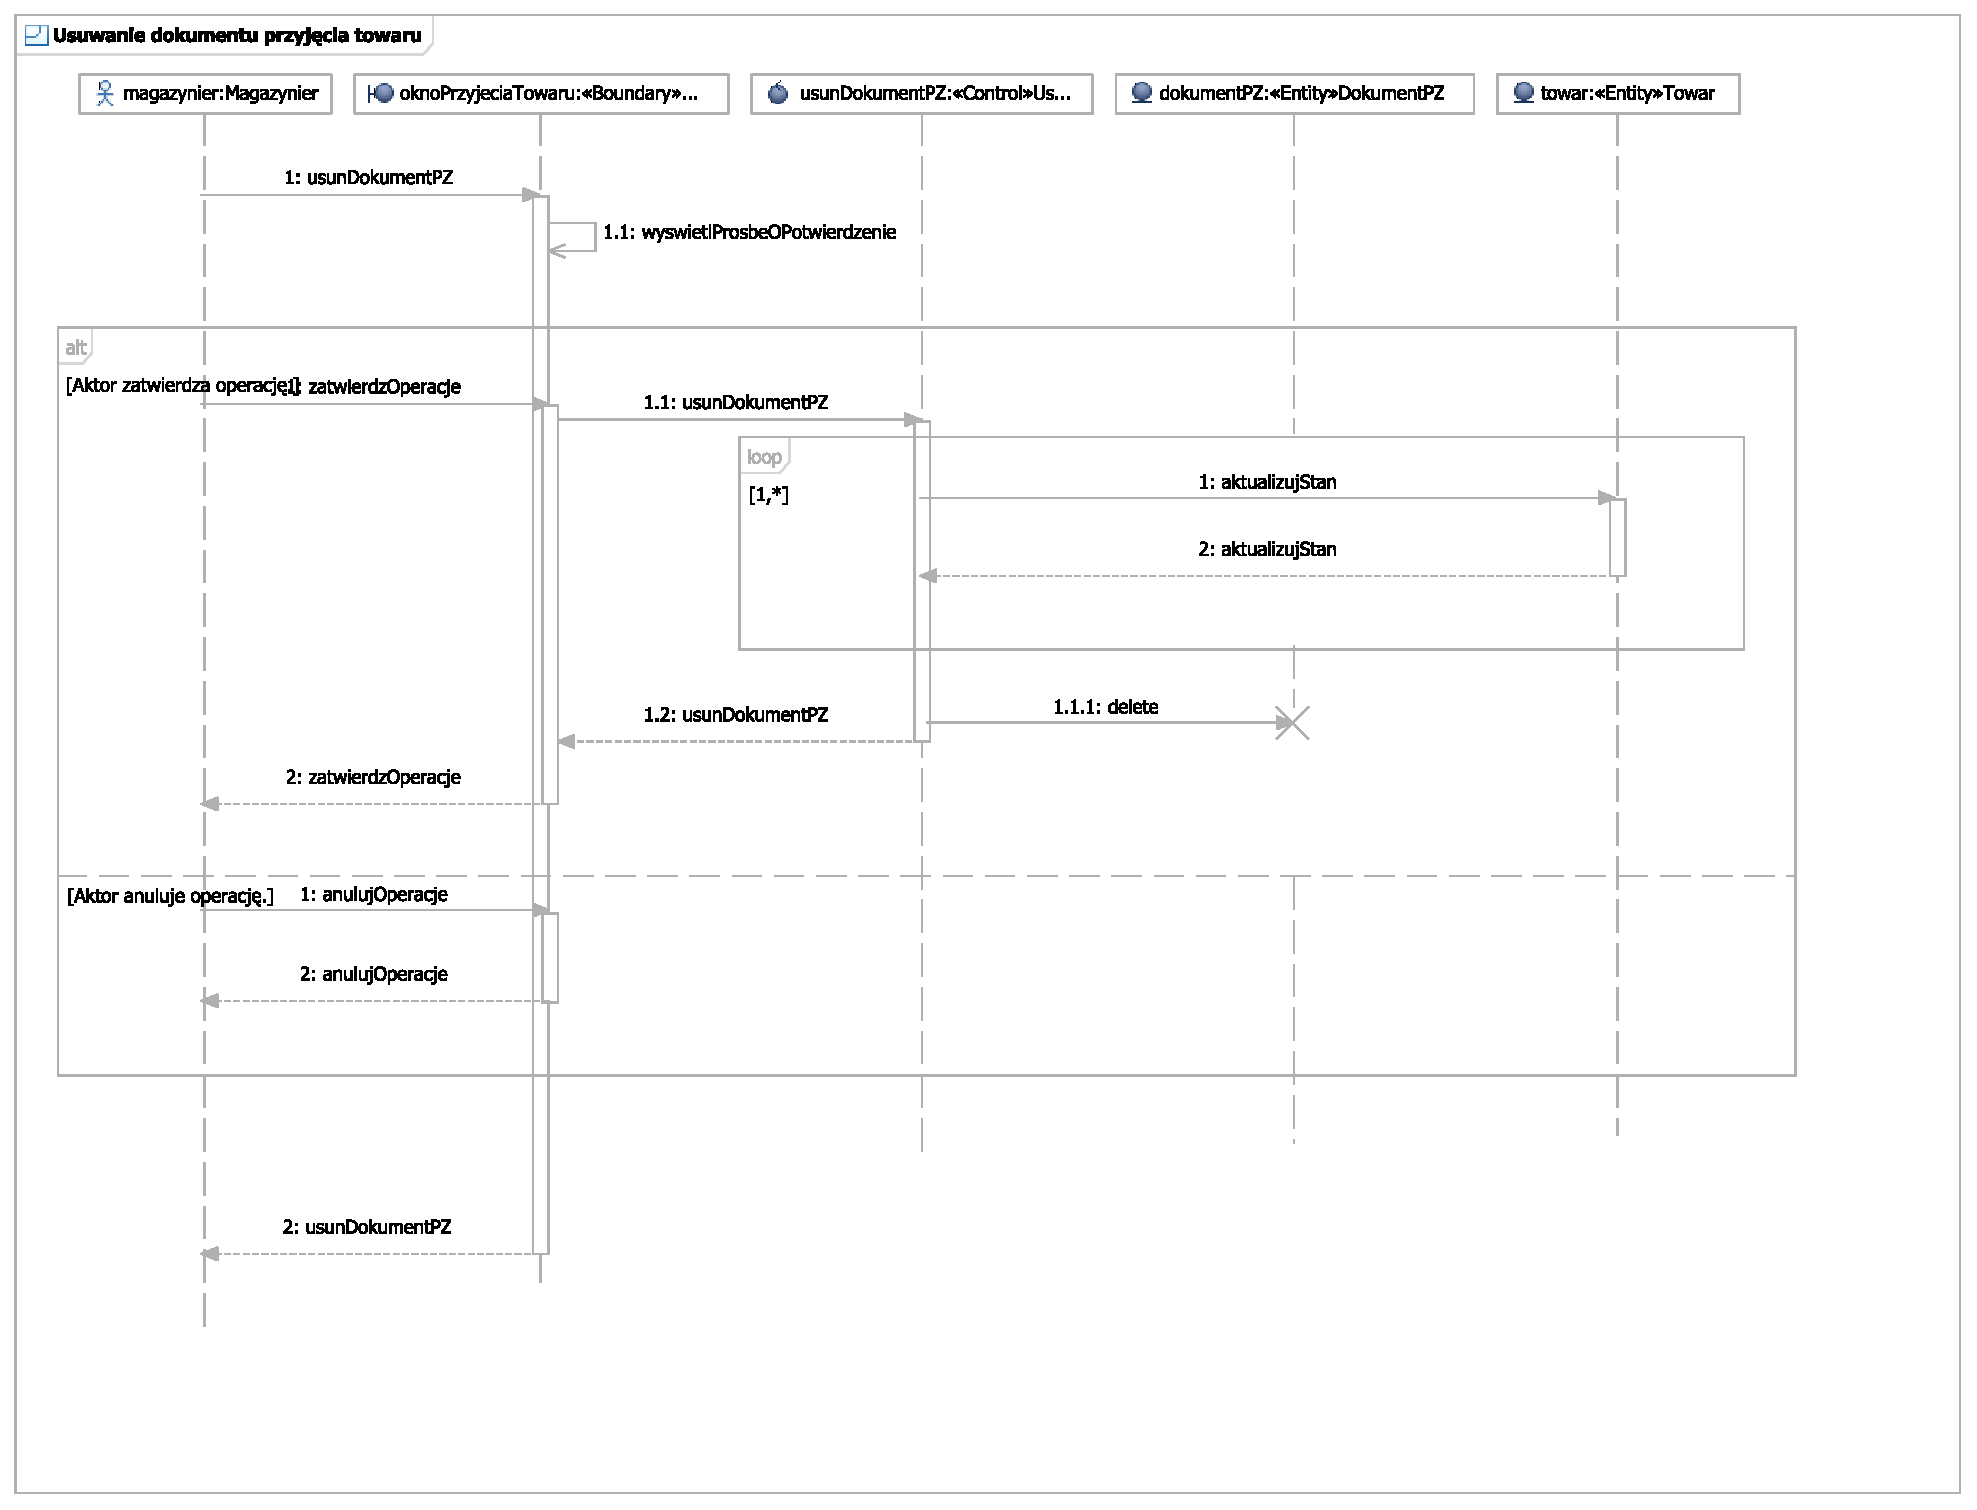
\includegraphics[angle=\seqangle, scale=0.5]{../img/usecase/pu26seq.pdf}
  \caption{\seqcaption26}
\end{figure}
\newpage

\subsection{Realizacja przyjęcia towaru na magazyn}
\begin{usecase}
  \addtitle{PU27}{Realizacja przyjęcia towaru na magazyn}
  \addfield{Priorytet:}{wysoki}
  \addfield{Aktor główny:}{Magazynier}
  \addfield{Rozszerza przypadki:}{PU23, PU24}
  \additemizedfield{Warunki początkowe:}{
    \item Aktor został uwierzytelniony.
    \item Wybrane przyjęcie towaru nie zostało jeszcze zrealizowane.}
  \additemizedfield{Warunki końcowe:} {
    \item Dokument przyjęcia towaru został oznaczony jako zrealizowany.
    \item Możliwe jest utworzenie korekty do zrealizowanego dokumentu przyjęcia towaru.
  }
  \addscenario{Scenariusz główny:}{
     \item Aktor wybiera opcję przyjęcia towaru na magazyn.
     \item System prosi o potwierdzenie realizacji przyjęcia towaru na magazyn.
     \item Aktor potwierdza realizację przyjęcia towaru na magazyn.
     % TODO mogło by być np powiadomienie dla dostawcy, że towar został przyjęty.
     \item System oznacza dokument przyjęcia towaru jako zrealizowany.
  }
 \addscenario{Scenariusz alternatywny:}{
    \item[4.a] Aktor anuluje realizację przyjęcia towaru.
      \begin{enumerate}
        \item[1.--2.] Jak w scenariuszu głównym.
        \item[3.] Aktor anuluje realizację dokumentu.
        \item[4.] System wyświetla informację, że operacja została anulowana.
      \end{enumerate}
  }
  \addfield{Wymagania funkcjonalne:}{4.4}
\end{usecase}

\begin{figure}[H]
  \centering
  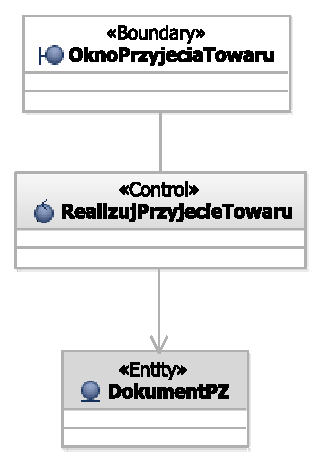
\includegraphics[angle=\ecbangle, scale=\ecbscale]{../img/usecase/pu27ecb.pdf}
  \caption{\ecbcaption27}
\end{figure}

\begin{figure}[H]
  \centering
  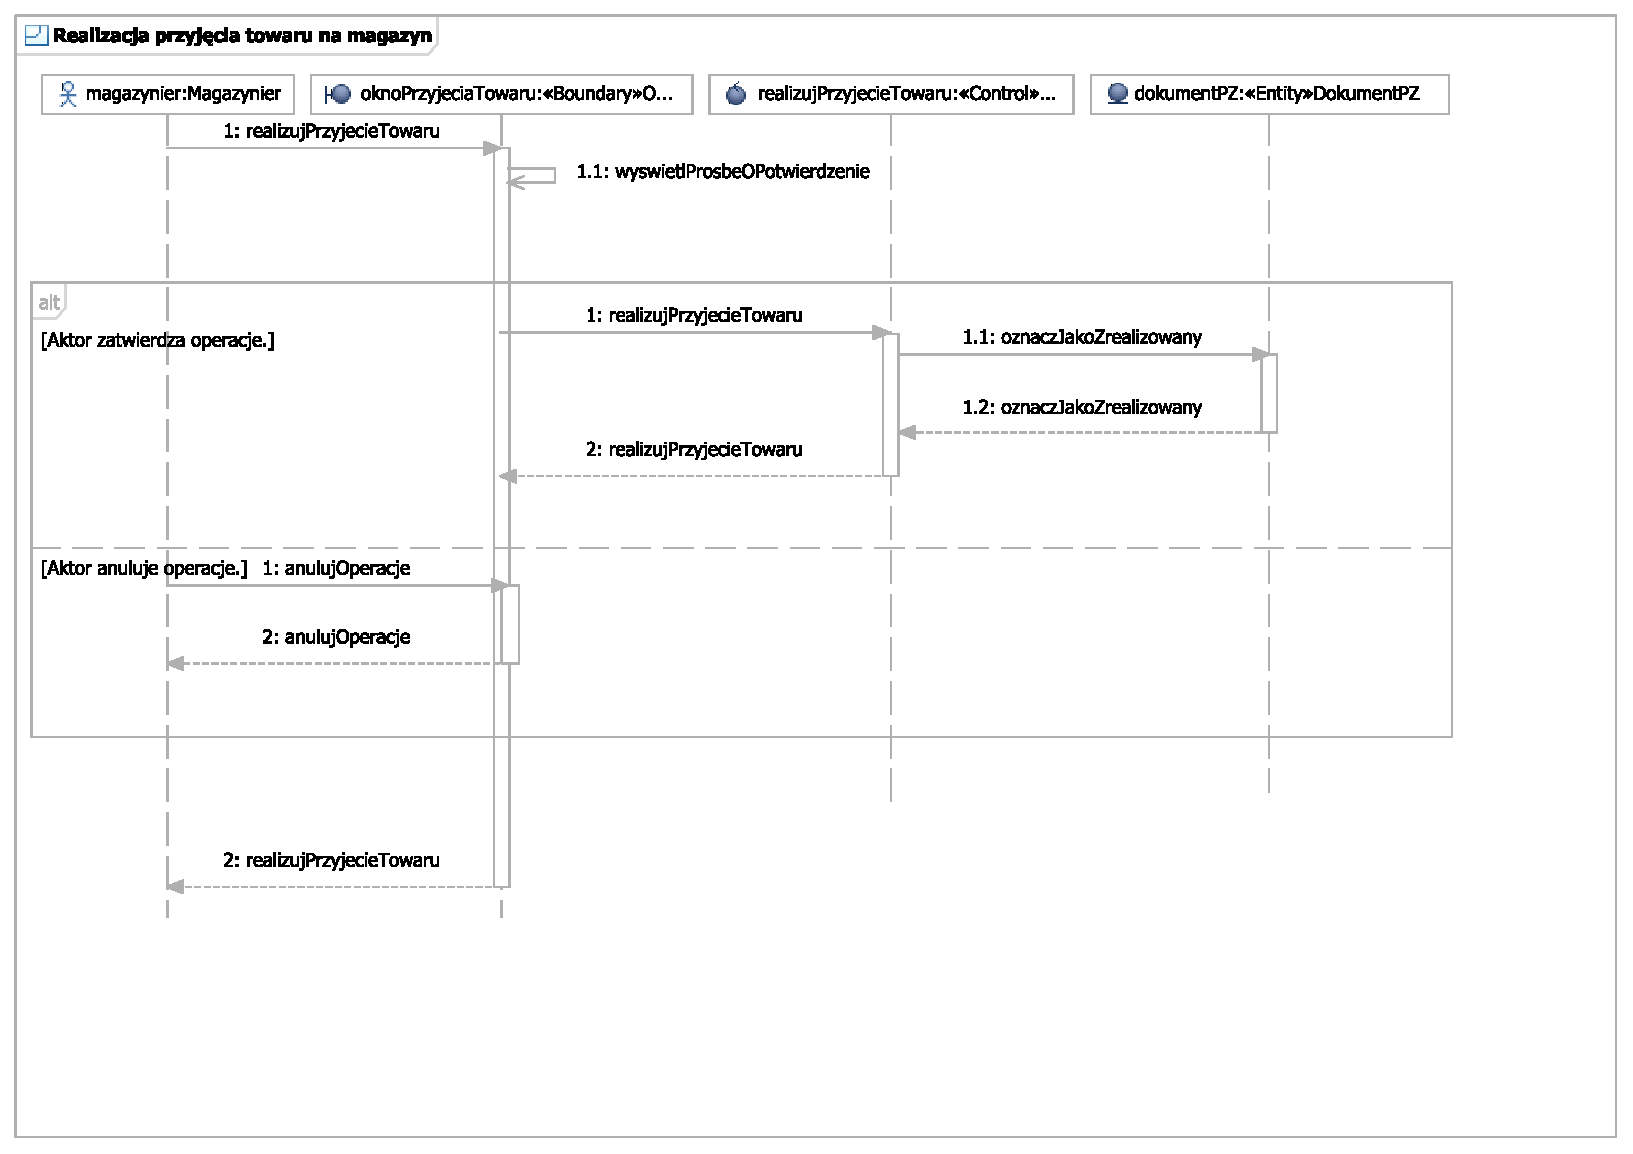
\includegraphics[angle=\seqangle, scale=\seqscale]{../img/usecase/pu27seq.pdf}
  \caption{\seqcaption27}
\end{figure}
\newpage

\subsection{Korekta przyjęcia towaru}
\begin{usecase}
  \addtitle{PU28}{Korekta przyjęcia towaru}
  \addfield{Priorytet:}{wysoki}
  \addfield{Aktor główny:}{Magazynier}
  \addfield{Rozszerza przypadki:}{PU23}
  \additemizedfield{Warunki początkowe:}{
     \item Aktor został uwierzytelniony.
     \item Wybrany dokument przyjęcia towaru został już zrealizowany.
  }
  \additemizedfield{Warunki końcowe:}{ 
    \item Dokument korekty przyjęcia towaru został zapisany w systemie.
    \item Ilość przechowywanych towarów została zaktualizowana zgodnie z wartością podaną na korekcie. 
    \item Ilość przechowywanego towaru jest zgodna z warunkami poprawności danych przedstawionymi w \ref{dziedzina-problemu}.
  }
  \addscenario{Scenariusz główny:}{
    \item Aktor wybiera opcję utworzenia korekty dla wskazanego dokumentu przyjęcia towaru.
    \item System wyświetla formularz nowej korekty. 
    \item Aktor wypełnia podstawowe dane korekty.
    \item Aktor wybiera towary, które podlegają zwrotowi oraz ich cenę.
    \item Aktor wybiera opcję zapisania korekty.
    \item System informuje aktora, że dane zostały poprawnie zaktualizowane.
  }
  \addscenario{Scenariusz alternatywny:} {
    \item [3.a] Aktor nie podał wymaganych pól formularza:
      \begin{enumerate}
        \item[1--4.] Jak w scenariuszu głównym.
        \item[5.] System wyświetla powiadomienie o konieczności podania wymaganych informacji.
        \item[6.] Aktor wraca do punktu 3.  
      \end{enumerate}
    \item [3.b] Aktor podał błędne wartości pól formularza:
      \begin{enumerate}
        \item[1--4.] Jak w scenariuszu głównym.
        \item[5.] System wyświetla powiadomienie o błędnych polach formularza.
        \item[6.] Aktor wraca do punktu 3.
      \end{enumerate}
     \item[5.a] Aktor wybrał ten sam towar co najmniej dwa razy.
       \begin{enumerate}
       \item[1--5.] Jak w scenariuszu głównym.
       \item[6.] System informuje aktora, że co najmniej dwa razy wybrał ten sam towar, podane ilości towaru zostaną więc zsumowane.
       \item[7.] System wyświetla zsumowane wartości dla tych samych towarów.
       \item[8--...] Jak w scenariuszu głównym.
       \end{enumerate}
  }
  \addfield{Zakres przetwarzanych danych:} {
    Pola dokumentu przyjęcia towaru takie jak przedstawione w rozdziale \ref{dziedzina-problemu}.
  }
  \addfield{Warunki poprawności danych:}{
    Warunki poprawności takie jak przedstawione w rozdziale \ref{dziedzina-problemu}.
  }
  \addfield{Wymagania funkcjonalne:}{4.5}
\end{usecase}

\begin{figure}[H]
  \centering
  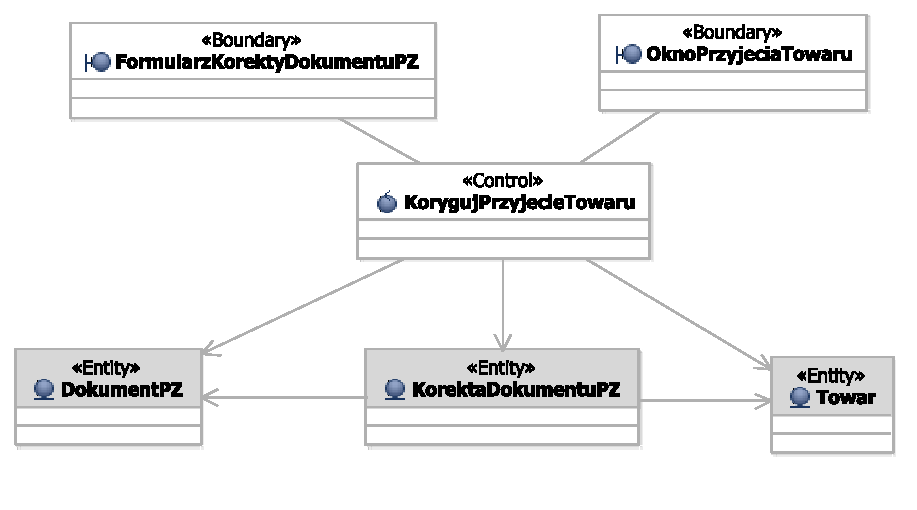
\includegraphics[angle=\ecbangle, scale=\ecbscale]{../img/usecase/pu28ecb.pdf}
  \caption{\ecbcaption28}
\end{figure}
\newpage
\begin{figure}[H]
  \centering
  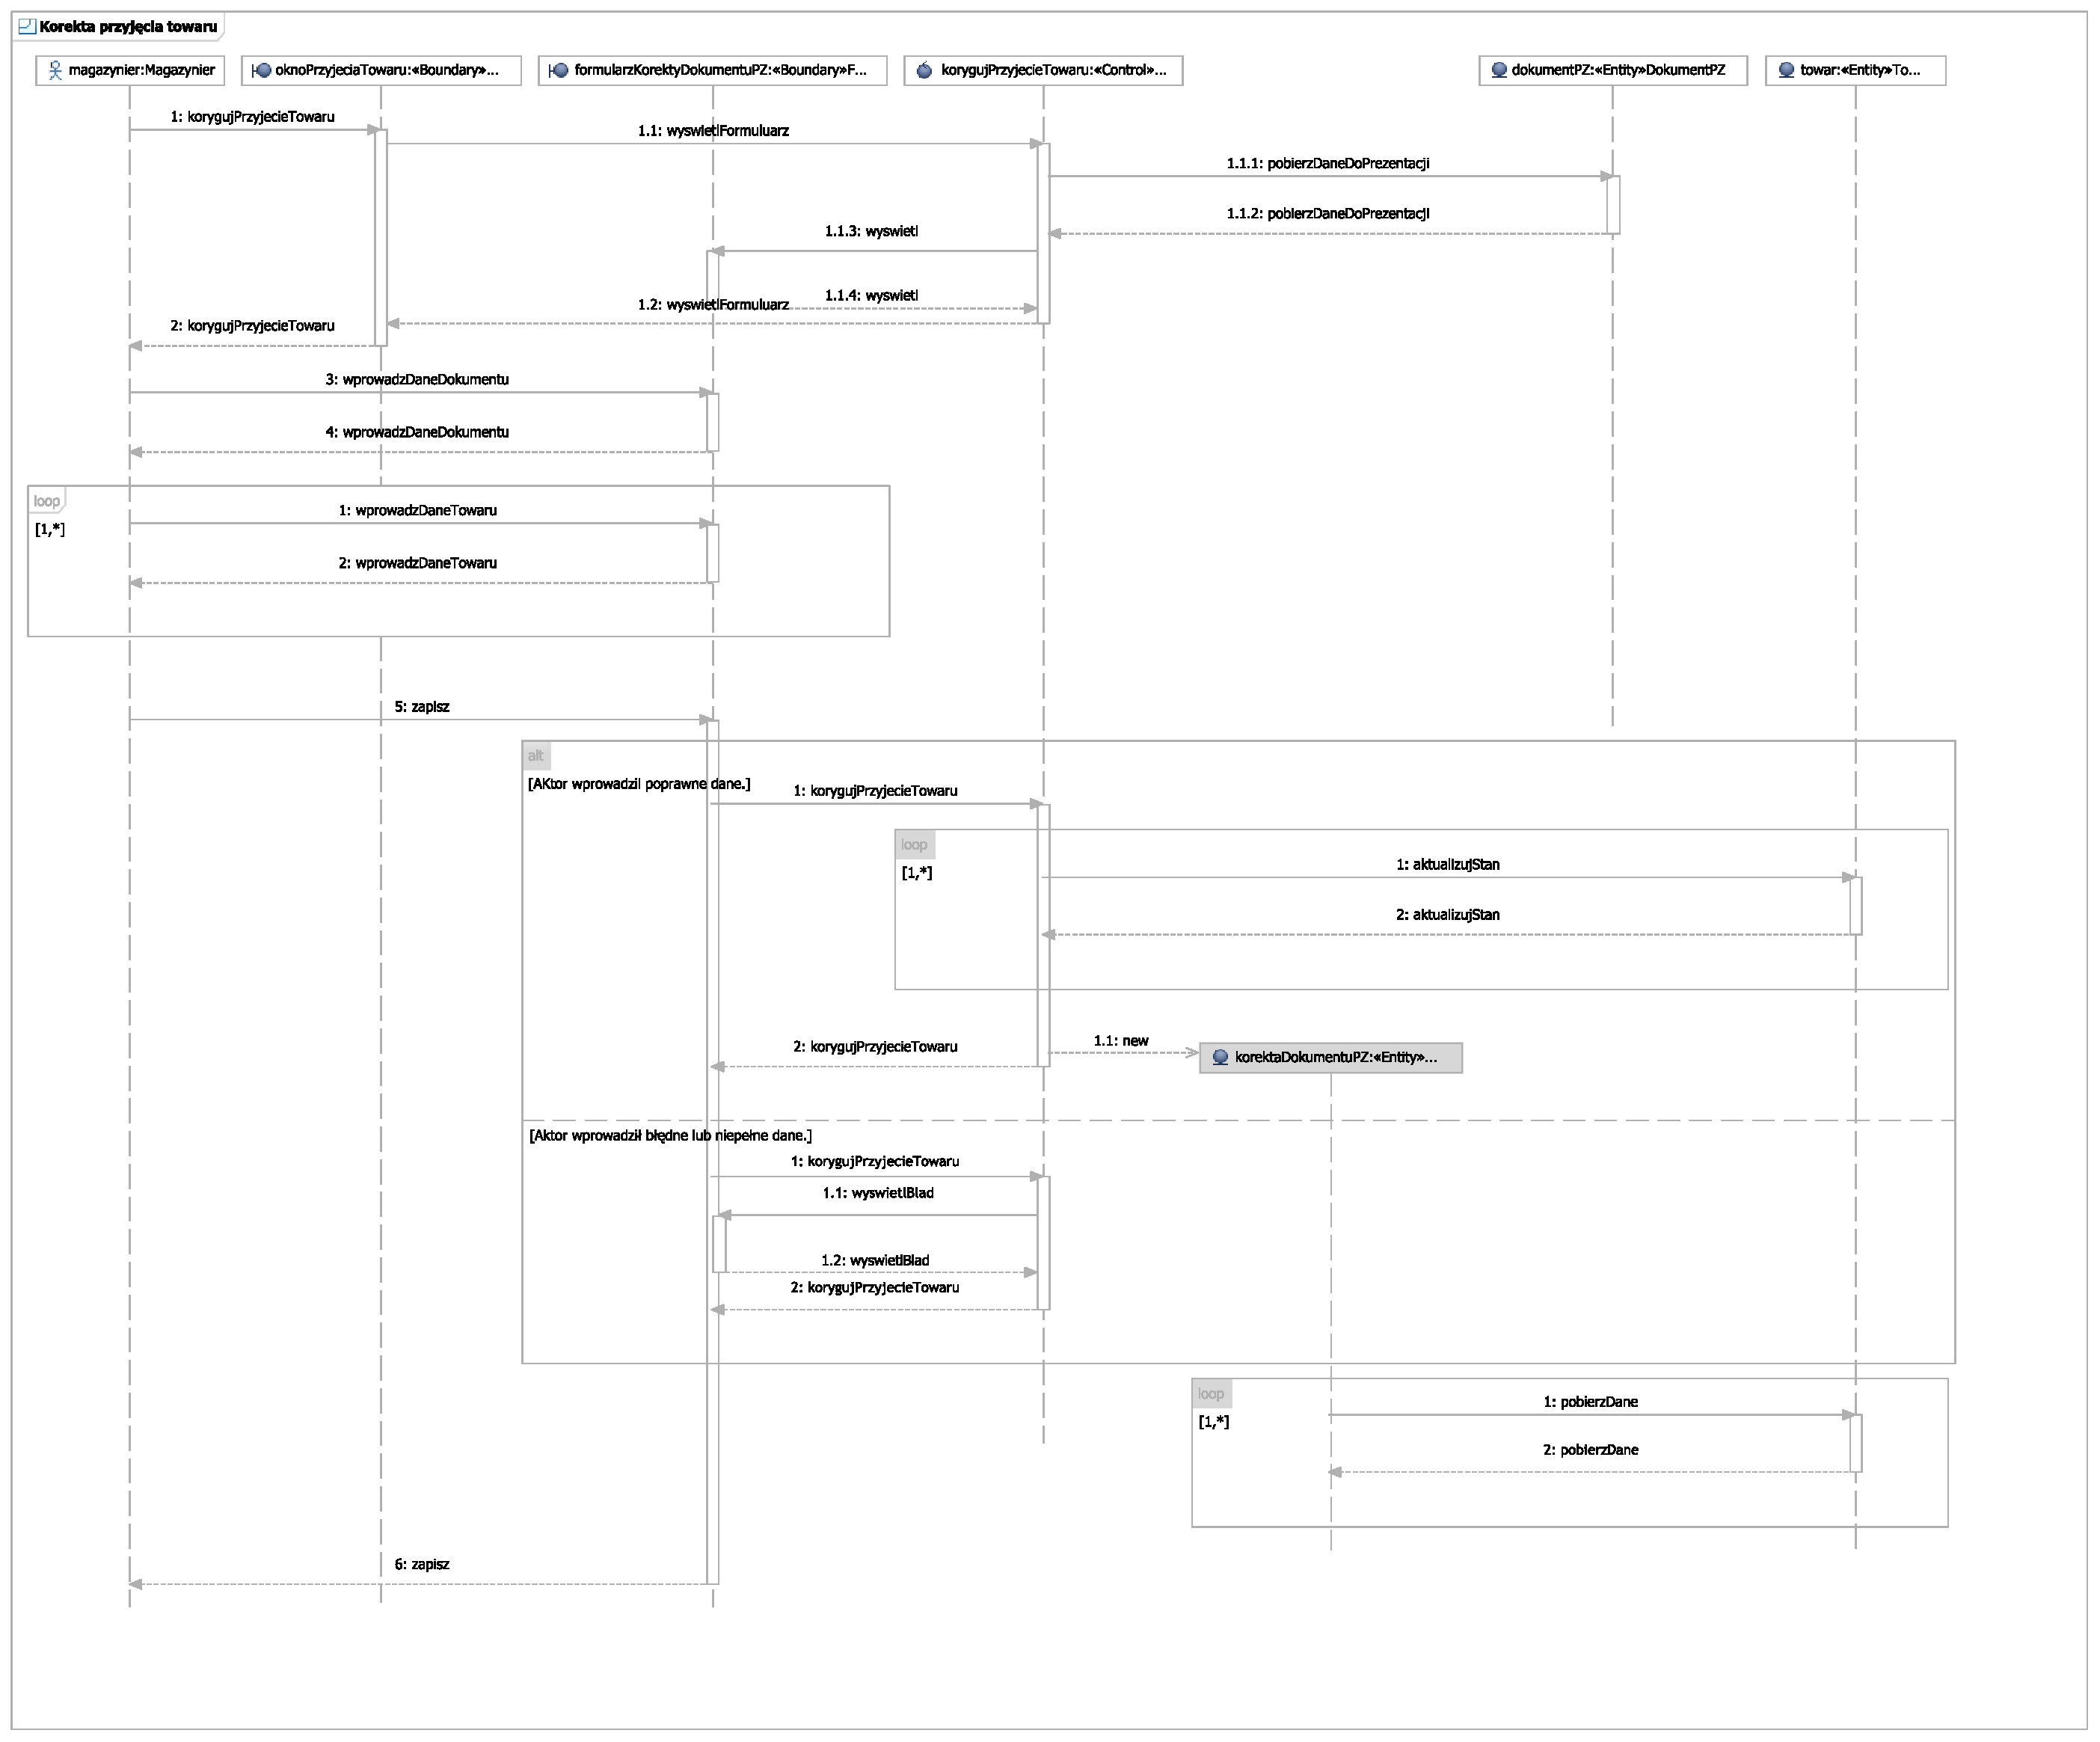
\includegraphics[angle=\seqangle, scale=0.35]{../img/usecase/pu28seq.pdf}
  \caption{\seqcaption28}
\end{figure}
\newpage






